% Options for packages loaded elsewhere
\PassOptionsToPackage{unicode}{hyperref}
\PassOptionsToPackage{hyphens}{url}
\PassOptionsToPackage{dvipsnames,svgnames,x11names}{xcolor}
%
\documentclass[
  11pt,
  a4paper,
]{krantz}
\usepackage{amsmath,amssymb}
\usepackage{iftex}
\ifPDFTeX
  \usepackage[T1]{fontenc}
  \usepackage[utf8]{inputenc}
  \usepackage{textcomp} % provide euro and other symbols
\else % if luatex or xetex
  \usepackage{unicode-math} % this also loads fontspec
  \defaultfontfeatures{Scale=MatchLowercase}
  \defaultfontfeatures[\rmfamily]{Ligatures=TeX,Scale=1}
\fi
\usepackage{lmodern}
\ifPDFTeX\else
  % xetex/luatex font selection
    \setmonofont[Scale=0.7]{Source Code Pro}
\fi
% Use upquote if available, for straight quotes in verbatim environments
\IfFileExists{upquote.sty}{\usepackage{upquote}}{}
\IfFileExists{microtype.sty}{% use microtype if available
  \usepackage[]{microtype}
  \UseMicrotypeSet[protrusion]{basicmath} % disable protrusion for tt fonts
}{}
\makeatletter
\@ifundefined{KOMAClassName}{% if non-KOMA class
  \IfFileExists{parskip.sty}{%
    \usepackage{parskip}
  }{% else
    \setlength{\parindent}{0pt}
    \setlength{\parskip}{6pt plus 2pt minus 1pt}}
}{% if KOMA class
  \KOMAoptions{parskip=half}}
\makeatother
\usepackage{xcolor}
\usepackage[margin=27mm]{geometry}
\usepackage{longtable,booktabs,array}
\usepackage{calc} % for calculating minipage widths
% Correct order of tables after \paragraph or \subparagraph
\usepackage{etoolbox}
\makeatletter
\patchcmd\longtable{\par}{\if@noskipsec\mbox{}\fi\par}{}{}
\makeatother
% Allow footnotes in longtable head/foot
\IfFileExists{footnotehyper.sty}{\usepackage{footnotehyper}}{\usepackage{footnote}}
\makesavenoteenv{longtable}
\usepackage{graphicx}
\makeatletter
\def\maxwidth{\ifdim\Gin@nat@width>\linewidth\linewidth\else\Gin@nat@width\fi}
\def\maxheight{\ifdim\Gin@nat@height>\textheight\textheight\else\Gin@nat@height\fi}
\makeatother
% Scale images if necessary, so that they will not overflow the page
% margins by default, and it is still possible to overwrite the defaults
% using explicit options in \includegraphics[width, height, ...]{}
\setkeys{Gin}{width=\maxwidth,height=\maxheight,keepaspectratio}
% Set default figure placement to htbp
\makeatletter
\def\fps@figure{htbp}
\makeatother
\setlength{\emergencystretch}{3em} % prevent overfull lines
\providecommand{\tightlist}{%
  \setlength{\itemsep}{0pt}\setlength{\parskip}{0pt}}
\setcounter{secnumdepth}{5}
% definitions for citeproc citations
\NewDocumentCommand\citeproctext{}{}
\NewDocumentCommand\citeproc{mm}{%
  \begingroup\def\citeproctext{#2}\cite{#1}\endgroup}
\makeatletter
 % allow citations to break across lines
 \let\@cite@ofmt\@firstofone
 % avoid brackets around text for \cite:
 \def\@biblabel#1{}
 \def\@cite#1#2{{#1\if@tempswa , #2\fi}}
\makeatother
\newlength{\cslhangindent}
\setlength{\cslhangindent}{1.5em}
\newlength{\csllabelwidth}
\setlength{\csllabelwidth}{3em}
\newenvironment{CSLReferences}[2] % #1 hanging-indent, #2 entry-spacing
 {\begin{list}{}{%
  \setlength{\itemindent}{0pt}
  \setlength{\leftmargin}{0pt}
  \setlength{\parsep}{0pt}
  % turn on hanging indent if param 1 is 1
  \ifodd #1
   \setlength{\leftmargin}{\cslhangindent}
   \setlength{\itemindent}{-1\cslhangindent}
  \fi
  % set entry spacing
  \setlength{\itemsep}{#2\baselineskip}}}
 {\end{list}}
\usepackage{calc}
\newcommand{\CSLBlock}[1]{\hfill\break\parbox[t]{\linewidth}{\strut\ignorespaces#1\strut}}
\newcommand{\CSLLeftMargin}[1]{\parbox[t]{\csllabelwidth}{\strut#1\strut}}
\newcommand{\CSLRightInline}[1]{\parbox[t]{\linewidth - \csllabelwidth}{\strut#1\strut}}
\newcommand{\CSLIndent}[1]{\hspace{\cslhangindent}#1}

%%
\usepackage{booktabs}
\usepackage{longtable}
\usepackage[bf,singlelinecheck=off]{caption}
%\usepackage{animate} %%% SEE: https://stackoverflow.com/questions/30476119/plot-animation-in-knitr-rmarkdown: PDF animations
\usepackage{times,pifont} % Nice fonts
\usepackage{fancyhdr}
\usepackage{tabularx} % For column specifications, using the kable_styling function  column_spec()
\usepackage{tabu} % For column specifications, using the kable_styling function  column_spec()
\usepackage{float} % Needed for some kableExtra stuff
\usepackage{mdframed}
\usepackage{enumitem} % To change the itemize spacing in exercises.
\usepackage{subfig} % For sub-figure captions
%\usepackage{caption} % Reformat captions
\usepackage[font={small,it}]{caption}

% FIGURE PLACEMENT: https://tex.stackexchange.com/questions/140568/how-to-set-default-positioning-of-figure-table-document-wide
\makeatletter
  \providecommand*\setfloatlocations[2]{\@namedef{fps@#1}{#2}}
\makeatother
\setfloatlocations{figure}{hbtp}
\setfloatlocations{table}{hbtp}


%\setmainfont[UprightFeatures={SmallCapsFont=AlegreyaSC-Regular}]{Alegreya}

\usepackage{framed,color}
\definecolor{shadecolor}{RGB}{224,224,224}
\definecolor{lightshadecolor}{RGB}{230, 230, 255}
\definecolor{textcolor}{RGB}{124,124,124}

\definecolor{exampleExtraColor}{RGB}{209, 223, 250}
\definecolor{examplecolor}{RGB}{240, 240, 240}

\renewcommand{\textfraction}{0.05}
\renewcommand{\topfraction}{0.8}
\renewcommand{\bottomfraction}{0.8}
\renewcommand{\floatpagefraction}{0.75}

%\renewenvironment{quote}{\begin{VF}}{\end{VF}}
\renewenvironment{quote}%
{\begin{kframe}}
{\end{kframe}}

\usepackage{hyperref}
\let\oldhref\href
\renewcommand{\href}[2]{#2\footnote{\url{#1}}}

\ifxetex
  \usepackage{letltxmacro}
  \setlength{\XeTeXLinkMargin}{1pt}
  \LetLtxMacro\SavedIncludeGraphics\includegraphics
  \def\includegraphics#1#{% #1 catches optional stuff (star/opt. arg.)
    \IncludeGraphicsAux{#1}%
  }%
  \newcommand*{\IncludeGraphicsAux}[2]{%
    \XeTeXLinkBox{%
      \SavedIncludeGraphics#1{#2}%
    }%
  }%
\fi

% Default figure width
\setkeys{Gin}{width=0.5\linewidth}


\makeatletter
\newenvironment{kframe}{%
\medskip{}
\setlength{\fboxsep}{.8em}
 \def\at@end@of@kframe{}%
 \ifinner\ifhmode%
  \def\at@end@of@kframe{\end{minipage}}%
  \begin{minipage}{\columnwidth}%
 \fi\fi%
 \def\FrameCommand##1{\hskip\@totalleftmargin \hskip-\fboxsep
 \colorbox{shadecolor}{##1}\hskip-\fboxsep
     % There is no \\@totalrightmargin, so:
     \hskip-\linewidth \hskip-\@totalleftmargin \hskip\columnwidth}%
 \MakeFramed {\advance\hsize-\width
   \@totalleftmargin\z@ \linewidth\hsize
   \@setminipage}}%
 {\par\unskip\endMakeFramed%
 \at@end@of@kframe}
\makeatother

\makeatletter
\@ifundefined{Shaded}{
}{\renewenvironment{Shaded}{\begin{kframe}}{\end{kframe}}}
\makeatother





\newenvironment{rmdthinkHTML}{}{}

\newenvironment{rmdblock}[1]
  {\setlength{\itemindent}{10em}\begin{quote}\vspace{-1em}
  \begin{itemize}\setlength{\parskip}{2mm}
  \renewcommand{\labelitemi}{
    \raisebox{-.5\height}[0pt][0pt]{
      {\setkeys{Gin}{width=1.5em,keepaspectratio}\includegraphics{icons/#1}}
    }
  }
  \setlength{\fboxsep}{1em}
  \begin{kframe}
  \item
  }
  {
  \end{kframe}
  \end{itemize}\vspace{-0.75em}\end{quote}
  }
\newenvironment{rmdblockNOIMAGE}
  {\begin{quote}\vspace{-0.75em}
  \setlength{\parskip}{2mm}
  %\begin{kframe}
  }
  {%\end{kframe}
  \vspace{-0.05em}\end{quote}
  }
  


\newenvironment{rmdobjectives}
  {\begin{rmdblock}{iconmonstr-target-4-240}}
  {\end{rmdblock}}
\newenvironment{rmddatafile}
  {\begin{rmdblock}{iconmonstr-download-8-240}}
  {\end{rmdblock}}
\newenvironment{rmdimportant}
  {\begin{rmdblock}{iconmonstr-warning-8-240}}
  {\end{rmdblock}}
\newenvironment{rmdtip}
  {\begin{rmdblock}{iconmonstr-info-6-240}}
  {\end{rmdblock}}



\newenvironment{darkgraytext}{\color{textcolor}}{\ignorespacesafterend}
%\AtBeginEnvironment{rmdblockNOIMAGE}{\begin{comment}}
%\AtEndEnvironment{rmdblockNOIMAGE}{\end{comment}}

%\usepackage{amsthm}
%\newtheorem*{ExampleFold}{Example}


%%% TRY HIDING EXAMPLE FOLDS, EXAMPLE FOLDS: To save paper in printing...???



% Redfine some existing environments
% -QUOTE
\makeatletter
\renewenvironment{quote}
               {\list{}{\vspace{-0.5em}\begin{kframe}\small%
                        \itemindent    \listparindent
                        \rightmargin   \leftmargin
                        \parsep        \z@ \@plus\p@}%
                \item\relax}
               {\end{kframe}\endlist}
\makeatother


% Change the lemma environment to be shaded
\usepackage{etoolbox}
\usepackage{framed}
\AtBeginEnvironment{lemma}{\begin{shaded}\begin{quote}\vspace{-2em}\setlength{\parskip}{6pt}} % Order must be shaded, then quote
\AtEndEnvironment{lemma}{\end{quote}\end{shaded}}


% ORIGINAL:
%\newenvironment{fold}
%  {\begin{rmdblock}{iconmonstr-idea-12-240}\vspace{-1em}\begin{darkgraytext}\footnotesize \textbf{Answer:}}
%  {\end{darkgraytext}\end{rmdblock}}
\newenvironment{fold}
  {\vspace{-6pt}\begin{rmdblockNOIMAGE}\begin{darkgraytext}\scriptsize \textbf{Answer:}}
  {\end{darkgraytext}\end{rmdblockNOIMAGE}}
  
% Change the  fold  environment to be disappeared
% Note: In the LaTeX code, it appears like this: \BeginKnitrBlock{fold}
%\usepackage{comment}
%\AtBeginEnvironment{fold}{\begin{comment}}
%\AtEndEnvironment{fold}{\end{comment}}

%\begin{shaded}}
%\AtEndEnvironment{fold}{\end{shaded}}

%%% IF ONLY THIS WORKED:
% \usepackage{comment}
% \includecomment{fold}


%%% Two column chunks: from https://github.com/grantmcdermott/two-col-test/blob/master/preamble.css
\usepackage{multicol}
%% Note: Pandoc (which is doing all of the output conversion behind the scenes) does not parse the content of LaTeX environments. This creates problems when you try to include LaTeX commands with curly brackets directly in your Rmd file. E.g. You can't just use `\begin{multicols}{2}` directly in your Rmd file. Luckily, a straightforward workaround is to simply define some new shortcut commands yourself as per the below.
%% See: https://stackoverflow.com/questions/25849814/rstudio-rmarkdown-both-portrait-and-landscape-layout-in-a-single-pdf/27334272#27334272
\newcommand{\btwocol}{\begin{multicols}{2}}
\newcommand{\etwocol}{\end{multicols}}
            

\usepackage{makeidx}
\makeindex

\urlstyle{tt}


% NOTE:  clashes with  ntheorem  package... if I want top use that. I tried to use if to put lemma in shaded backgrounds... without luck. So I just put this code back.
\usepackage{amsthm}
\makeatletter
\def\thm@space@setup{%
  \thm@preskip=8pt plus 2pt minus 4pt
  \thm@postskip=\thm@preskip
}

\makeatother



\frontmatter

%%% Turn off maketitle to get pdf image as title page (https://stackoverflow.com/questions/45963505/coverpage-and-copyright-notice-before-title-in-r-bookdown):
\let\oldmaketitle\maketitle
\AtBeginDocument{\let\maketitle\relax}

\usepackage{animate}
\ifLuaTeX
  \usepackage{selnolig}  % disable illegal ligatures
\fi
\usepackage{bookmark}
\IfFileExists{xurl.sty}{\usepackage{xurl}}{} % add URL line breaks if available
\urlstyle{same}
% Make links footnotes instead of hotlinks:
\DeclareRobustCommand{\href}[2]{#2\footnote{\url{#1}}}
\hypersetup{
  pdftitle={Science Research Methods: Software},
  pdfauthor={Peter K. Dunn},
  colorlinks=true,
  linkcolor={Maroon},
  filecolor={Maroon},
  citecolor={Blue},
  urlcolor={Blue},
  pdfcreator={LaTeX via pandoc}}

\title{Science Research Methods: Software}
\usepackage{etoolbox}
\makeatletter
\providecommand{\subtitle}[1]{% add subtitle to \maketitle
  \apptocmd{\@title}{\par {\large #1 \par}}{}{}
}
\makeatother
\subtitle{An introduction to quantitative research and statistics: Using software}
\author{Peter K. Dunn}
\date{Last updated: March 17, 2025}

\begin{document}
\maketitle



%\killtitle % Removes the title 

%\cleardoublepage\newpage\thispagestyle{empty}\null
%\cleardoublepage\newpage\thispagestyle{empty}\null
%\cleardoublepage\newpage
\thispagestyle{empty}
%\begin{center}
%\includegraphics{images/dedication.pdf}
%\end{center}

\makebox[\textwidth]{
\includegraphics[width=\paperwidth]{images/cover-Software}}
%\centerline{\includegraphics[width=\textwidth,height=\textheight]{images/cover.png}}

% Reinstate maketitle (https://stackoverflow.com/questions/45963505/coverpage-and-copyright-notice-before-title-in-r-bookdown):
\let\maketitle\oldmaketitle
\maketitle


\setlength{\abovedisplayskip}{-5pt}
\setlength{\abovedisplayshortskip}{-5pt}

%%% Footer
%\pagestyle{fancy}
%\fancyfoot[L]{\textit{Scientific Research Methods}}


%%% REDEFINE some environments

%%% BASED ONL
%%%   https://stackoverflow.com/questions/58195679/how-can-i-redefine-a-standard-bookdown-theorem-environment-in-latex-pdf (I asked)
%% and adapted using:
%%%   https://stackoverflow.com/questions/1565988/making-a-small-modification-to-a-latex-environment







\let\origexample=\example
\def\example{\begingroup\begin{quote}\setlength{\parskip}{3mm}\vspace{-7mm}\origexample}  
   %% -7mm removes some spacing at the top, which looked odd. Chosen by trial and error
   %% parskip added, otherwise no gap between paras in examples which looked odd.
\let\origendexample=\endexample
\def\endexample{\origendexample\end{quote}\endgroup}


\let\origdefinition=\definition
\def\definition{\begingroup\begin{quote}\vspace{-5mm}\origdefinition}  
   %% -5mm removes some spacing at the top, which looked odd. Chosen by trial and error
\let\origenddefinition=\enddefinition
\def\enddefinition{\origenddefinition\end{quote}\endgroup}


% \let\origlemma=\lemma
% \def\lemma{\begingroup\begin{quote}\vspace{-5mm}\origlemma\normalfont}  
%    %% -5mm removes some spacing at the top, which looked odd. Chosen by trial and error
% \let\origendlemma=\endlemma
% \def\endlemma{\origendlemma\end{quote}\endgroup}
% \renewenvironment{lemma}
%    {\begin{rmdthink}}
%    {\end{rmdthink}}







%%% Greyed background for lemma (now called Think)
% This works, but of course looses all the "lemma" stuff, like numbering and corss-referencing
%\renewenvironment{lemma}
%    {\begin{quote}}
%    {\end{quote}}


% Fix the itemize/enumerate spacing in exercises:
\let\origexercise=\exercise
\def\exercise{\begingroup\setitemize{labelindent=1.5em,labelsep=3mm,leftmargin=*}\setenumerate{labelindent=1.5em,labelsep=3mm,leftmargin=*}\origexercise}  
   %% -5mm removes some spacing at the top, which looked odd. Chosen by trial and error
\let\origendexercise=\endexercise
\def\endexercise{\origendexercise\endgroup}
   %% \setitem  from the  enumitem  package




% Exercise environment does not do dot points correctly: It does this:
%
%   1. This is the
%   way they are done.
%   No hanging pars
%
% So make some adjustments... but it is when itemize is called.


%\renewenvironment{example}[1]%
%  {\begin{quote}\textbf{#1:}}
%  {\end{quote}}

{
\hypersetup{linkcolor=}
\setcounter{tocdepth}{2}
\tableofcontents
}
\chapter*{Preface}\label{preface}


This book has been prepared for use with the book
\emph{Scientific Research and Methodology},
which is an introduction to quantitative research methods in the scientific, engineering and health disciplines.

This book introduces the whole research process, from asking a research question to analysis and reporting of the data.
The focus, however, is on the analysis of data.

\section*{Statistical software}\label{statistical-software}


This manual explains how to conduct some of the analyses in the book \href{https://bookdown.org/pkaldunn/SRM-Textbook/}{\emph{Scientific Research Method}} using software.
We discuss using \href{https://www.jamovi.org/}{jamovi} (\citeproc{ref-Software:jamovi}{The jamovi Project, n.d.}) and \href{https://www.ibm.com/products/spss-statistics}{SPSS} (\citeproc{ref-Software:SPSS}{IBM Corp 2016}) only.

jamovi is \emph{free} and is like (but not exactly the same as) SPSS.
From the \href{https://www.jamovi.org/}{jamovi homepage (sic)}:

\begin{quote}
jamovi is a new `3rd generation' statistical spreadsheet.
designed from the ground up to be easy to use, jamovi is a compelling alternative to costly statistical products such as SPSS and SAS.
\end{quote}

\section*{Callouts used on this book}\label{callouts-used-on-this-book}


The following callouts are used in this book:

\begin{rmdobjectives}
These chunks introduce the objectives for the chapters of the book.
\end{rmdobjectives}

\begin{rmdtip}
These chunks offer helpful information.
\end{rmdtip}

\begin{rmdimportant}
These chunks highlight common mistakes or warnings, about a particular concept or about using a formula.
\end{rmdimportant}

\begin{rmddatafile}
These chunks point to the data files being used, collated in Sect. \ref{DataFiles}, so you can download the data, and follow the instructions.
\end{rmddatafile}

\section*{Using statistical software rather than a spreadsheet}\label{using-statistical-software-rather-than-a-spreadsheet}


(The following information is based on (\citeproc{ref-mypapers:ScientificResearch}{Dunn 2025}).)

Many people use spreadsheets (such as Microsoft Excel) rather than statistical software.
But using spreadsheets requires extreme care; many extremely expensive and dangerous errors have been made through using spreadsheets (\citeproc{ref-altarawneh2017pilot}{AlTarawneh and Thorne 2017}), including problems \href{https://www.zdnet.com/article/excel-errors-microsofts-spreadsheet-may-be-hazardous-to-your-health/}{when reporting the 2020 COVID-19 pandemic}.

These problems emerge for different reasons:

\begin{itemize}
\tightlist
\item
  Spreadsheets often change the entered data (for example, reformatting entries as dates if the spreadsheet \emph{thinks} the data should be a date) in the interest of being `user-friendly', even when not appropriate.
  This has had dire consequences (\citeproc{ref-ziemann2016gene}{Ziemann, Eren, and El-Osta 2016}).
\item
  Many spreadsheets have errors in formulas (\citeproc{ref-panko1998hitting}{R. R. Panko and Sprague Jr 1998}), but these are incredible difficult to locate and hence fix (Galletta et al. (\citeproc{ref-galletta1996spreadsheet}{1996}), R. Panko (\citeproc{ref-panko2016we}{2016})).
\item
  Spreadsheets do not leave a record of how the data have been analysed; for example, formulas can be very difficult to understand and parse.
  Keeping a record of the analysis, new variables that have been created, and other operations with the data is called \hyperref[ReproducibleResearch]{\textbf{reproducible research}}.
  Reproducibility ensures, among other advantages, that the results can be checked by others.
\item
  Excel has bugs (Keeling and Pavur (\citeproc{ref-keeling2004numerical}{2004}), Mélard (\citeproc{ref-melard2014accuracy}{2014})) even in very basic operations (Berger (\citeproc{ref-berger2007nonstandard}{2007}), Hargreaves and McWilliams (\citeproc{ref-hargreaves2010polynomial}{2010})).
  After trying to fix these bugs, sometimes they are made even worse (\citeproc{ref-mccullough2002accuracy}{McCullough and Wilson 2002}).
\end{itemize}

Spreadsheets can be used for research and analysis\ldots{} but you must be very careful!
Many of the problems are due to human error, and some emerge because Excel is being used for purposes it is not really designed for (i.e.~scientific analysis).

\subsubsection*{Using jamovi and SPSS}\label{using-jamovi-and-spss}


\subsection*{jamovi}\label{jamovi}


We \textbf{strongly recommend} installing the \href{https://www.jamovi.org/download.html}{most recent \textbf{stable}, \textbf{desktop} (not online) version of jamovi}.

\subsection*{SPSS}\label{spss}


All recent versions of SPSS work in similar ways.
SPSS is installed in computer labs and available using \href{https://anywhere.usc.edu.au/vpn/index.html}{\emph{USC Anywhere}}.

\section*{Learning Outcomes}\label{learning-outcomes}


In this book, you will learn to:

\begin{itemize}
\tightlist
\item
  Use jamovi to conduct chi-square tests.
\item
  Use jamovi to conduct two-sample \(t\)-tests.
\item
  Use jamovi to create graphs.
\item
  Use SPSS to conduct chi-square tests.
\item
  Use SPSS to conduct two-sample \(t\)-tests.
\item
  Use SPSS to create graphs.
\end{itemize}

\section*{How to cite this book}\label{how-to-cite-this-book}


Peter K. Dunn (2019). \emph{Scientific Research Methods: Software manual}.
\url{https://bookdown.org/pkaldunn/SRM-software/}

\mainmatter

\chapter{Introduction}\label{introduction}

\textbf{Before} you start to use jamovi or SPSS, you need to know \emph{why} you need the software.

\begin{itemize}
\tightlist
\item
  If your RQ concerns the \textbf{relationship between two qualitative variables}:

  \begin{itemize}
  \tightlist
  \item
    Analysis of \textbf{odds ratios} using, for example, a \(\chi^2\)-test; or
  \item
    Analysis of \textbf{two proportions} using, for example, a \(z\)-test.
  \item
    Displays using a side-by-side or stacked barchart.
  \end{itemize}
\item
  If your RQ concerns the \textbf{difference between means in two groups}:

  \begin{itemize}
  \tightlist
  \item
    Analysis of two means using, for example, a two-sample \(t\)-test.
  \item
    Displays using a error bar chart (and perhaps a boxplot).
  \end{itemize}
\end{itemize}

The data files used in this document are available in Sect. \ref{DataFiles}.

You can download the data, and follow the instructions in this document.

\part{Using jamovi}\label{part-using-jamovi}

\chapter{jamovi: general information}\label{jamoviGeneral}

\begin{rmdobjectives}
\textbf{Topics} covered in this chapter:

\begin{itemize}
\tightlist
\item
  Tips for working with jamovi.
\end{itemize}
\end{rmdobjectives}

Before starting analysis with \href{https://www.jamovi.org/}{jamovi} (\citeproc{ref-Software:jamovi}{The jamovi Project, n.d.}), here are some \textbf{general tips}:

\begin{itemize}
\tightlist
\item
  jamovi is a very new package (built on R (\citeproc{ref-Software:Rsoftware}{R Core Team 2025})), and currently lacks some desirable features.
  These will no doubt arrive in due time.
\item
  jamovi is \textbf{free} to download, from \href{https://www.jamovi.org/}{the jamovi webpage}.
\item
  \emph{Except for graphs}, jamovi output should \textbf{not} be presented in reports or presentations.\\
  Instead, the information from jamovi output should be used to construct proper tables, or to produce proper conclusions.
\item
  The information about the variables must be correctly set up \textbf{before} analysis.
\item
  In jamovi (as with most statistical software), \emph{each row represents one unit of analysis}.
\item
  In jamovi (as with most statistical software), \emph{each column represents one variable}.
\item
  At the top of each column (but \textbf{not} in Row 1!) is the \emph{name} of the variable; \emph{double click} on the variable name and set information about the variables there (Fig. \ref{fig:jamoviVariables1}).
  Then you can tell jamovi information about the variables, such as whether the data are nominal, ordinal or `continuous' (which is what jamovi calls \emph{all} quantitative variables\ldots), and the \emph{levels} of the nominal and ordinal variables (Fig. \ref{fig:jamoviVariablesSet}).
\item
  You can get help with using jamovi by:

  \begin{itemize}
  \tightlist
  \item
    Watching software screencasts on Canvas.
  \item
    Using \href{https://www.jamovi.org/user-manual.html}{jamovi resources}.
  \item
    Using \href{https://www.linkedin.com/learning/}{LinkedIn Learning}.
  \item
    Watching \href{https://datalab.cc/tools/jamovi}{videos}.
  \item
    Asking SCI110 staff \textbf{in tutorials}, or in the Canvas \emph{Discussions}.
  \end{itemize}
\end{itemize}

\begin{figure}[hbtp]

{\centering 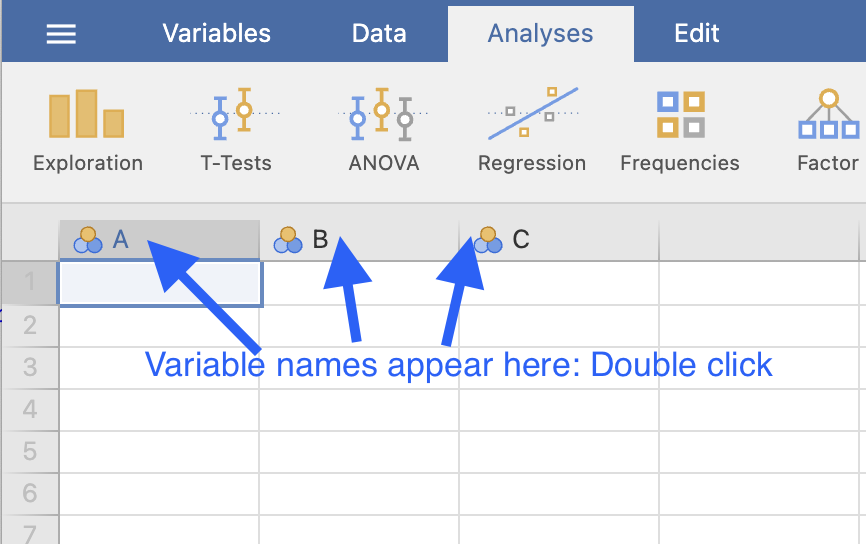
\includegraphics[width=0.5\linewidth]{jamoviImages/jamovi-Vars2} 

}

\caption{Click on the column headers to describe the variables}\label{fig:jamoviVariables1}
\end{figure}

\begin{figure}[hbtp]

{\centering 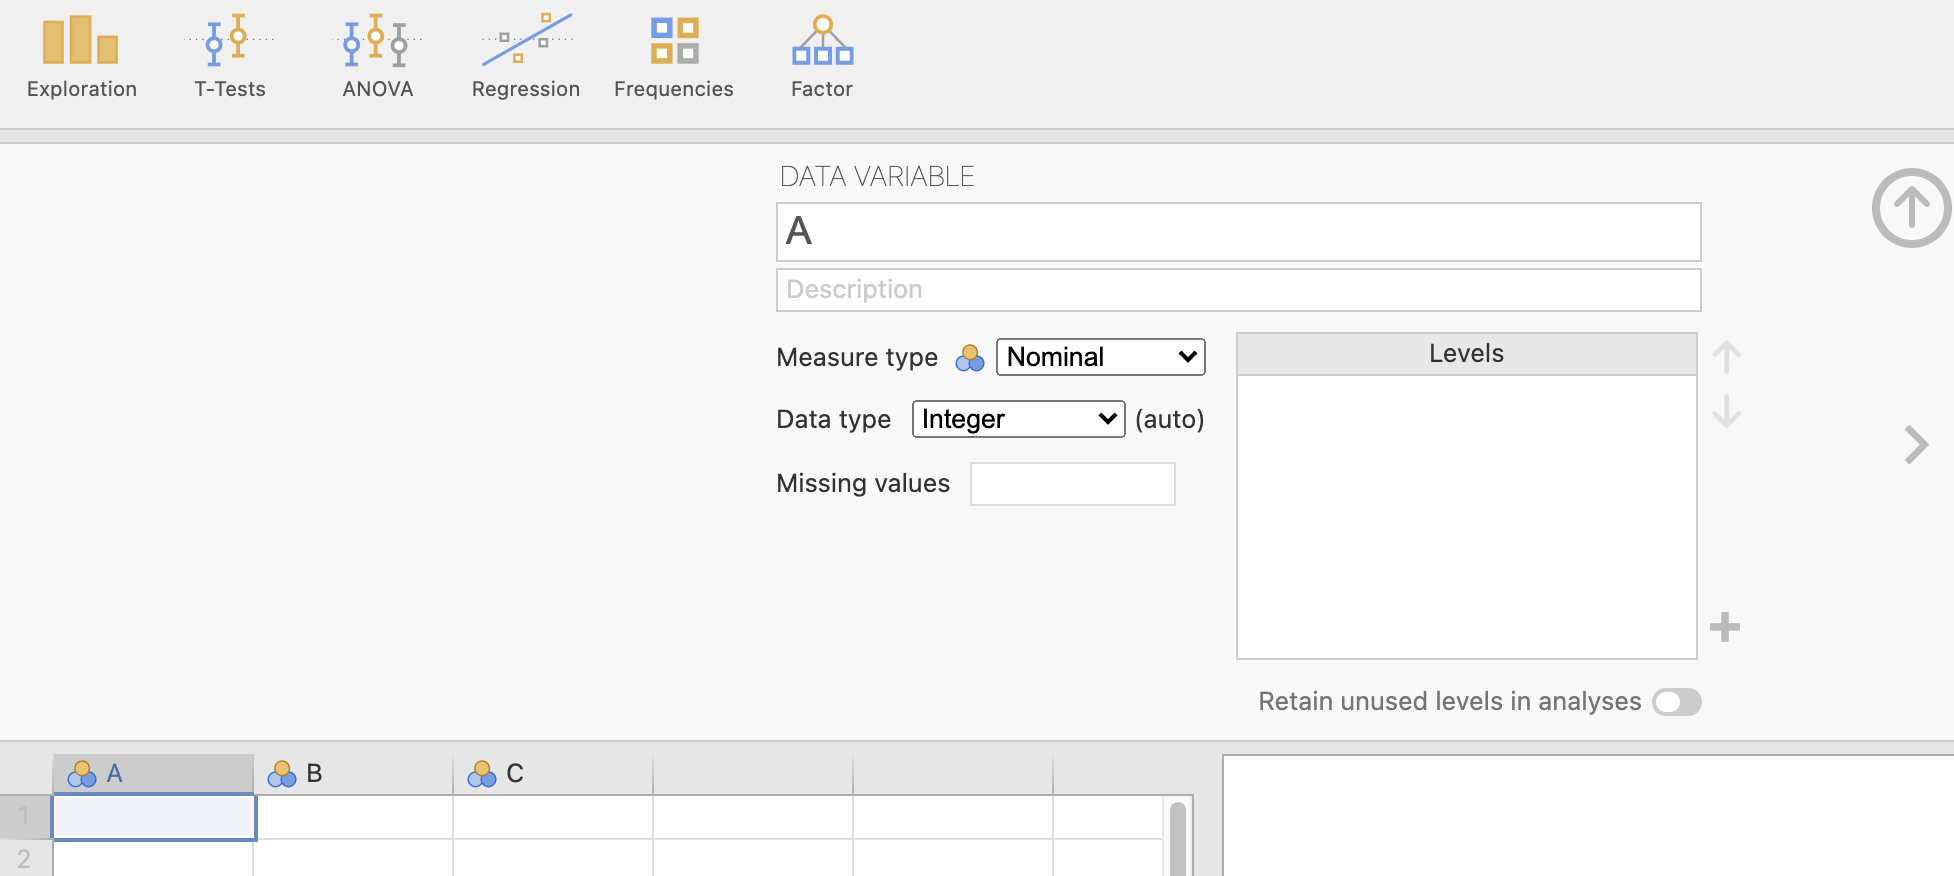
\includegraphics[width=1\linewidth]{jamoviImages/jamovi-VarSet} 

}

\caption{The information to fill in for each variable}\label{fig:jamoviVariablesSet}
\end{figure}

\chapter{jamovi: inference for two odds or two proportions}\label{jamoviChisquare}

\begin{rmdobjectives}
\textbf{Topics} covered in this chapter:

\begin{itemize}
\tightlist
\item
  How to use jamovi for comparing two odds (i.e., analysis using odds ratios).
\item
  How to use jamovi for comparing two proportions.
\end{itemize}
\end{rmdobjectives}

\section{Introduction}\label{B12Data}

RQs comparing \emph{two qualitative variables} require count data that can be compiled into a two-way table of counts.
Consider data (\citeproc{ref-data:Gammon2012:B12}{Gammon et al. 2012}) \href{https://bookdown.org/pkaldunn/SRM-Textbook/AnalysisOddsRatio.html}{in Exercise~31.16 of the textbook} (Table~\ref{tab:jamoviB12Data}).

\begin{rmddatafile}
The data file (\texttt{B12-Long.csv}) can be downloaded in Sect. \ref{DataFiles}.
You can download the data, and follow the instructions.
\end{rmddatafile}

\textbf{This data set is available from the textbook as \texttt{B12-Long}} in
\href{https://bookdown.org/pkaldunn/SRM-Textbook/AppendixDataSets.html}{Appendix~A}.
You can download the data and follow along if you wish.

There are \emph{two qualitative variables} being measured on each individual:

\begin{enumerate}
\def\labelenumi{\arabic{enumi}.}
\tightlist
\item
  Whether the person is vegetarian (or not);
\item
  Whether the person is B12 deficient (or not).
\end{enumerate}

Hence, jamovi will have \emph{two columns}: one for each variable.
There are \(124\) units of analysis, so there are \emph{\(124\) rows} of data.

\begin{table}
\centering
\caption{\label{tab:jamoviB12Data}The number of vegetarian and non-vegetarian women who are (and are not) B12 deficient}
\centering
\fontsize{10}{12}\selectfont
\begin{tabular}[t]{lrr>{}r}
\toprule
\textbf{ } & \textbf{B12 deficient} & \textbf{Not B12 deficient} & \textbf{Total}\\
\midrule
Vegetarians & 8 & 26 & \textbf{34}\\
Non-vegetarians & 8 & 82 & \textbf{90}\\
\midrule
\textbf{Total} & \textbf{16} & \textbf{108} & \textbf{\textbf{124}}\\
\bottomrule
\end{tabular}
\end{table}

\section{Data entry}\label{jamoviChiSquareDataEntry}

In jamovi, the two columns are set up as follows:

\begin{itemize}
\tightlist
\item
  \textbf{Diet}: \texttt{1} means `Vegetarian' (i.e.~in Row~1 of the data table), and \texttt{2} means `Non-vegetarian' (i.e.~in Row~2 of the data table in Table~\ref{tab:jamoviB12Data}).
\item
  \textbf{B12}: \texttt{1} means `B12 deficient' (i.e.~in Column~1 of the data table), and \texttt{2} means `\emph{Not} B12 deficient' (i.e.~in Column~2 of the data table in Table~\ref{tab:jamoviB12Data}); see Fig.~\ref{fig:jamoviChisqB12DataLong}.
\end{itemize}

The data needs to be set up so that \emph{each row represents one unit of analysis}.
That means there will be \(124\) rows of data: one for each person (unit of analysis).

In jamovi, the data are entered as shown in Fig.~\ref{fig:jamoviChisqB12DataLong}; there are \(124\)~rows, but we only show some of these rows to save space.

\begin{rmdimportant}
Each \emph{row} in the jamovi data represents one \emph{unit of analysis}.

Each \emph{column} in the jamovi data represents one \emph{variable}.
\end{rmdimportant}

\begin{figure}[hbtp]

{\centering 
\includegraphics[width=0.8\linewidth]{jamoviImages/Chisq/B12-Data-Long} 

}

\caption{The B12 data entered into jamovi}\label{fig:jamoviChisqB12DataLong}
\end{figure}

\begin{rmdimportant}
\textbf{Note that I entered \texttt{1} and \texttt{2} into the jamovi worksheet}:
jamovi just \emph{shows} what these mean in the worksheet, because I have told jamovi what the \texttt{1} and the \texttt{2} mean.
\end{rmdimportant}

Your data is now set up and ready to use.

\section{Analysis}\label{jamoviChiSquareAnalysis}

Remember that \textbf{this data set is available from the textbook as \texttt{B12-Long}} in \href{https://bookdown.org/pkaldunn/SRM-Textbook/AppendixDataSets.html}{Appendix~A}

Once the data are entered, we can begin analysis:

\begin{enumerate}
\def\labelenumi{\arabic{enumi}.}
\tightlist
\item
  \textbf{Use the menu:} select \textbf{Analyses\textgreater{} Frequencies\textgreater{} Independent samples (\(\chi^2\) test of association)}
\end{enumerate}

\begin{figure}[hbtp]

{\centering 
\includegraphics[width=0.6\linewidth]{jamoviImages/Chisq/B12-Menu2} 

}

\caption{Select the correct test}\label{fig:jamoviChisqB12Menu}
\end{figure}

\begin{enumerate}
\def\labelenumi{\arabic{enumi}.}
\setcounter{enumi}{1}
\tightlist
\item
  \textbf{Select the variables:} dragging them from the left panel to the \textbf{Rows} and \textbf{Columns} areas as appropriate.
  In Table~\ref{tab:jamoviB12Data}, \textbf{Diet} is in the rows of the table, for example.
\end{enumerate}

\begin{figure}[hbtp]

{\centering 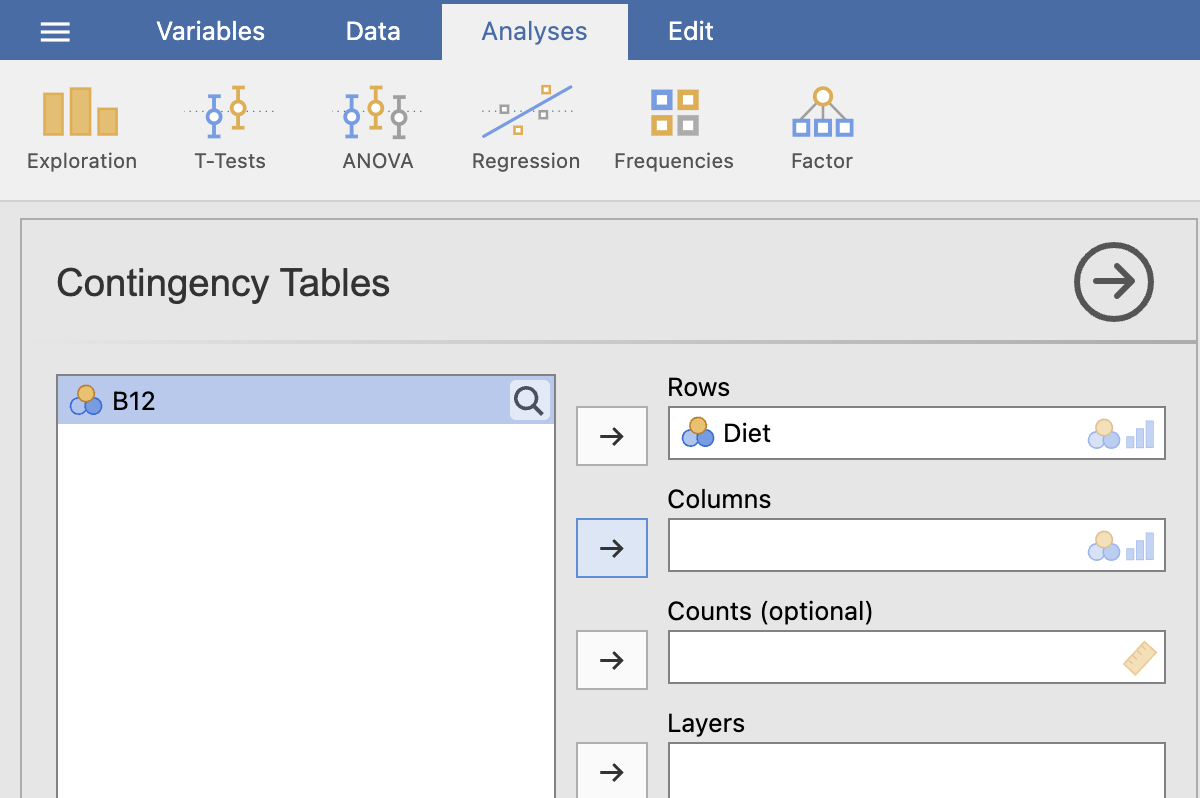
\includegraphics[width=0.5\linewidth]{jamoviImages/Chisq/B12-Analysis} 

}

\caption{Enter the variables}\label{fig:jamoviChisqB12Analysis}
\end{figure}

\begin{enumerate}
\def\labelenumi{\arabic{enumi}.}
\setcounter{enumi}{2}
\tightlist
\item
  \textbf{Select the analysis options:} Under the area where you entered the variables, select the right-pointing arrow beside \textbf{Statistics}, and then:
\end{enumerate}

\begin{itemize}
\tightlist
\item
  Select \texttt{X2}: this conducts the \(\chi^2\) hypothesis test for comparing odds.
\item
  Select \texttt{z\ test\ for\ difference\ in\ 2\ proportions}: this conducts the \(z\)-test to compare proportions.
\item
  Select \texttt{Odds\ ratio}: this shows the value of the odds ratio.
\item
  Select \texttt{Difference\ in\ proportions}: this shows the difference between the two proportions.
\item
  Select \texttt{Confidence\ intervals}: this shows the CI for the odds ratio, and for the difference between the proportions.
\end{itemize}

\begin{figure}[hbtp]

{\centering 
\includegraphics[width=0.6\linewidth]{jamoviImages/Chisq/B12-Analysis-Stats-Ticks} 

}

\caption{Check the correct options}\label{fig:jamoviChisqB12AnalysisStatsTicks}
\end{figure}

\begin{enumerate}
\def\labelenumi{\arabic{enumi}.}
\setcounter{enumi}{3}
\tightlist
\item
  You will have your output in the jamovi Output window on the right.
\end{enumerate}

\section{Numerical summaries}\label{jamoviChiSquareNumericalSummaries}

\emph{Percentages} can be obtained from the same place: \textbf{Analyses\textgreater{} Frequencies Independent samples (\(\chi^2\) test of association)}.
Under the area where you selected the \textbf{Statistics}, select the right-pointing arrow beside \textbf{Cells}, and then:

\begin{itemize}
\tightlist
\item
  Select \texttt{Row} under the \textbf{Percentages} section; and/or
\item
  Select \texttt{Column} under the \textbf{Percentages} section.
\end{itemize}

\begin{figure}[hbtp]

{\centering 
\includegraphics[width=0.6\linewidth]{jamoviImages/Chisq/B12-Analysis-Cells-Ticks} 

}

\caption{Select what to show in the table}\label{fig:jamoviChisqB12AnalysisCellsTicks}
\end{figure}

Of course, you can select any of the other options too, and see what happens.

\chapter{jamovi: inference about the difference between two means}\label{jamoviTwoSampleT}

\begin{rmdobjectives}
\textbf{Topics} covered in this tutorial:

\begin{itemize}
\tightlist
\item
  Learn how to use jamovi for comparing two means.
\end{itemize}
\end{rmdobjectives}

\section{Introduction}\label{jamoviLeanAngle}

Two independent sample \(t\)-tests are used to compare the means of two separate groups.

Consider the face-plant data (\citeproc{ref-data:Wojcik:ForwardFall}{Wojcik et al. 1999}) \href{https://bookdown.org/pkaldunn/SRM-Textbook/AnalysisTwoMeans.html}{used in Exercise~30.11 of the textbook} (Table~\ref{tab:jamoviFacePlant}).

\begin{rmddatafile}
The data file (\texttt{forwardfall.csv}) can be downloaded in Sect. \ref{DataFiles}.

You can download the data, and follow the instructions.
\end{rmddatafile}

\begin{table}
\centering
\caption{\label{tab:jamoviFacePlant}Lean-forward angles for older and younger women}
\centering
\fontsize{10}{12}\selectfont
\begin{tabular}[t]{ccc}
\toprule
\multicolumn{2}{c}{\textbf{Younger women }} & \multicolumn{1}{c}{\textbf{Older women }} \\
\cmidrule(l{3pt}r{3pt}){1-2} \cmidrule(l{3pt}r{3pt}){3-3}
29 & 34 & 18\\
32 & 27 & 15\\
34 & 32 & 23\\
31 & 28 & 13\\
33 & 27 & 12\\
\bottomrule
\end{tabular}
\end{table}

\section{Data entry}\label{jamoviTwoSampleDataEntry}

In the \textbf{Data} area, each row represents a unit of analysis (in this case, a person), as is usual in jamovi (Fig.~\ref{fig:jamoviTwotFacePlantData}).

Each unit of analysis gets two variables recorded: one is quantitative (\textbf{Lean angle (in degrees)}), and one is qualitative (\textbf{Age group}).
So there are two columns in the data, one for each variable.

The order of the variables doesn't matter, but here the quantitative variable is listed first (the lean-forward angle), and then the qualitative variable (the age group).

The variables need to be properly set up (by double-clicking on the variable names); see Figs.~\ref{fig:jamoviTwotFacePlantvarsAngle} and \ref{fig:jamoviTwotFacePlantAgegroup}.

\begin{figure}[hbtp]

{\centering 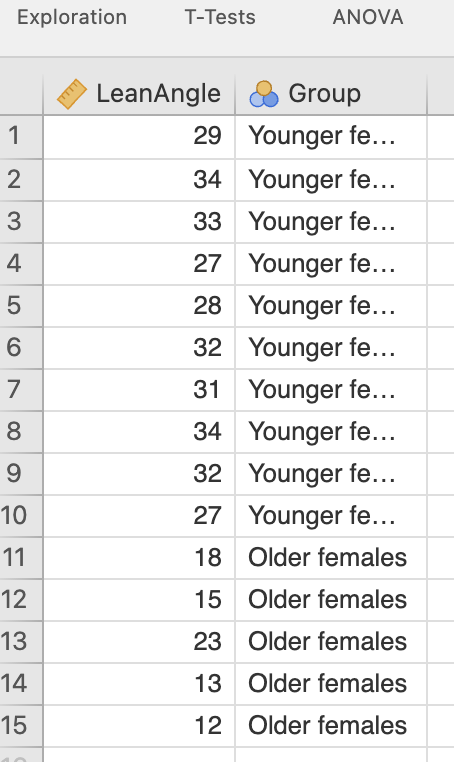
\includegraphics[width=0.3\linewidth]{jamoviImages/TwoInd/FacePlant-Data} 

}

\caption{The data entered in jamovi}\label{fig:jamoviTwotFacePlantData}
\end{figure}

\begin{figure}[hbtp]

{\centering 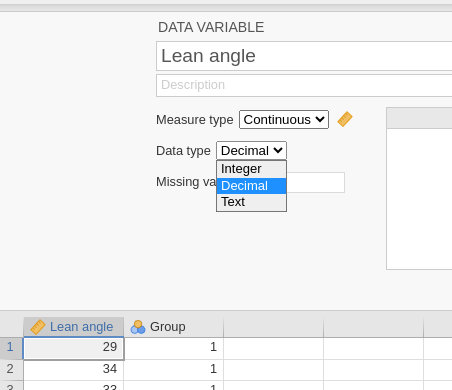
\includegraphics[width=0.7\linewidth]{jamoviImages/TwoInd/FacePlant-vars-Angle} 

}

\caption{Describing the quantitative variable}\label{fig:jamoviTwotFacePlantvarsAngle}
\end{figure}

\begin{figure}[hbtp]

{\centering 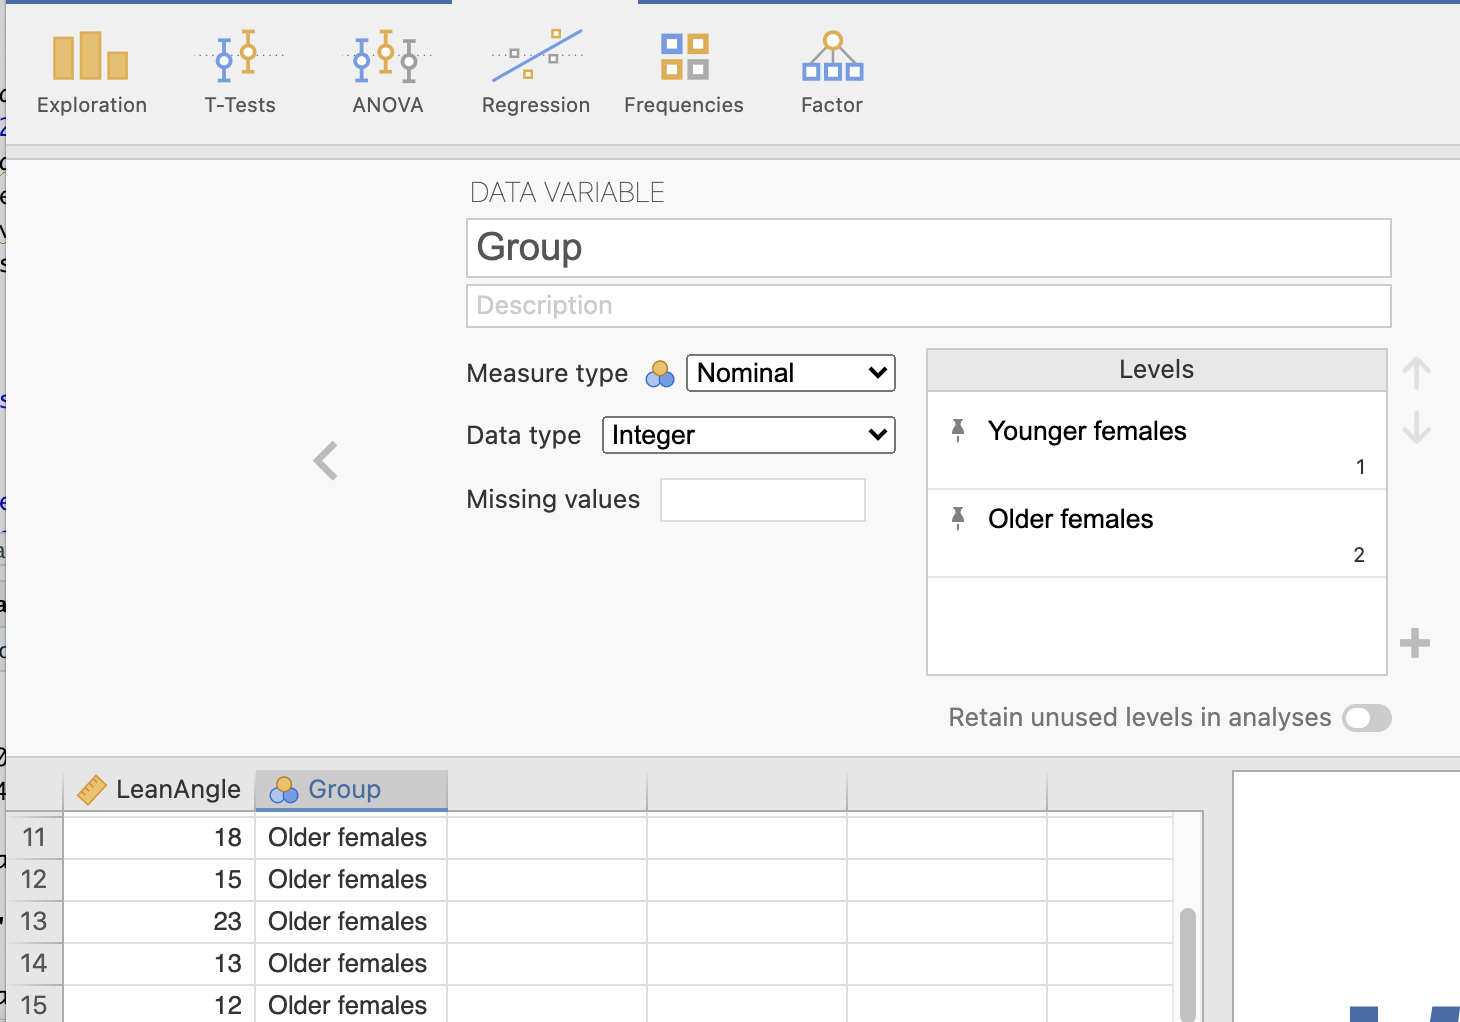
\includegraphics[width=0.7\linewidth]{jamoviImages/TwoInd/FacePlant-vars-Agegroup} 

}

\caption{Describing the qualitative variable}\label{fig:jamoviTwotFacePlantAgegroup}
\end{figure}

The two age groups are defined so that a \texttt{1} represents younger women, and a \texttt{2} represents older women.
In the jamovi worksheet, the values \texttt{1} and \texttt{2} were entered, but jamovi shows what these mean in the worksheet when these values are defined.

\section{Analysis}\label{jamoviTwoSampleAnalysis}

Remember, \textbf{this data set is available from the textbook as \texttt{forwardfall.csv}} in \href{https://bookdown.org/pkaldunn/SRM-Textbook/AppendixDataSets.html}{Appendix~A}.
You can download the data and follow along if you wish.

\begin{enumerate}
\def\labelenumi{\arabic{enumi}.}
\tightlist
\item
  \textbf{Use the jamovi menu}: select \textbf{Analyses\textgreater{} T-Tests\textgreater{} Independent Samples T-Test}
\item
  \textbf{Select the Variables}.

  \begin{itemize}
  \tightlist
  \item
    For the \textbf{Dependent Variables}, add the quantitative variable (here, \texttt{LeanAngle}).
  \item
    For the \textbf{Grouping Variable}, add the qualitative variable (here, \texttt{Group}).
  \end{itemize}
\item
  Then select the options:
\end{enumerate}

\begin{itemize}
\tightlist
\item
  \texttt{Student\textquotesingle{}s} and \texttt{Welch\textquotesingle{}s} should be select to perform the hypothesis test and compute the CIs.
\item
  \texttt{Mean\ difference} to show the difference between the two means in the output.
\item
  \texttt{Confidence\ interval} to show the CI for the difference between the two means.
\item
  \texttt{Descriptives} to show the numerical summary of each group.
\item
  \texttt{Descriptives\ plot} to show the error bar chart.
\end{itemize}

\begin{rmdimportant}
Even if you have a one-tailed hypothesis, keep the hypotheses as the two-tailed (first) option, or you will get some strange output.
The one-tailed \(P\)-value will be half the two-tailed \(P\)-value.
\end{rmdimportant}

\begin{figure}[hbtp]

{\centering 
\includegraphics[width=0.7\linewidth]{jamoviImages/TwoInd/FacePlant-TTest} 

}

\caption{Enter the variables}\label{fig:jamoviTwotFacePlant-TTest}
\end{figure}

\begin{enumerate}
\def\labelenumi{\arabic{enumi}.}
\setcounter{enumi}{3}
\tightlist
\item
  You will have your output in the jamovi Output window.
\end{enumerate}

\section{Numerical summaries}\label{jamoviTwoSampleNumericalSummaries}

The \emph{mean}, \emph{median}, \emph{standard deviation} and \emph{standard error} of each group
are produced as part of the output
from the \(t\)-test analysis step above.

The \emph{mean} and \emph{standard error} for the \emph{difference}
is obtained from the \(t\)-test output too.

\chapter{jamovi: graphs}\label{jamoviGraphs}

\begin{rmdobjectives}
\textbf{Topics} covered in this tutorial:

\begin{itemize}
\tightlist
\item
  Creating graphs in jamovi.
\end{itemize}
\end{rmdobjectives}

\begin{rmddatafile}
The data files used in this section can be downloaded in Sect. \ref{DataFiles}.

You can download the data, and follow the instructions.
\end{rmddatafile}

Graphs in jamovi are sometimes produced as part of the \textbf{Analyses},
and sometimes through the \textbf{Exploration} menu.

\section{Bar charts (side-by-side; stacked)}\label{jamoviSideBySide}

For this section,
the data introduced in Sect. \ref{B12Data} are used.

\begin{enumerate}
\def\labelenumi{\arabic{enumi}.}
\tightlist
\item
  \textbf{Use the jamvoi menu:} select \textbf{Analyses\textgreater{} Frequencies\textgreater{} Independent samples (\(\chi^2\) test of association)}.
\item
  \textbf{Add the variables}.
  Add the variables to the rows and columns (in this case, the \texttt{Rows} is \texttt{Diet} and the \texttt{Columns} is \texttt{B12}).
\item
  Click on the right-pointing arrow next to the \textbf{Plots} option from the bottom of the left-side screen.
\item
  In the \textbf{Plots} section, select \texttt{Bar\ Plot}; then select \textbf{Bar Type} (either a \texttt{Side\ by\ side} bar chart, or a \texttt{Stacked} bar chart).
\end{enumerate}

\begin{figure}[hbtp]

{\centering 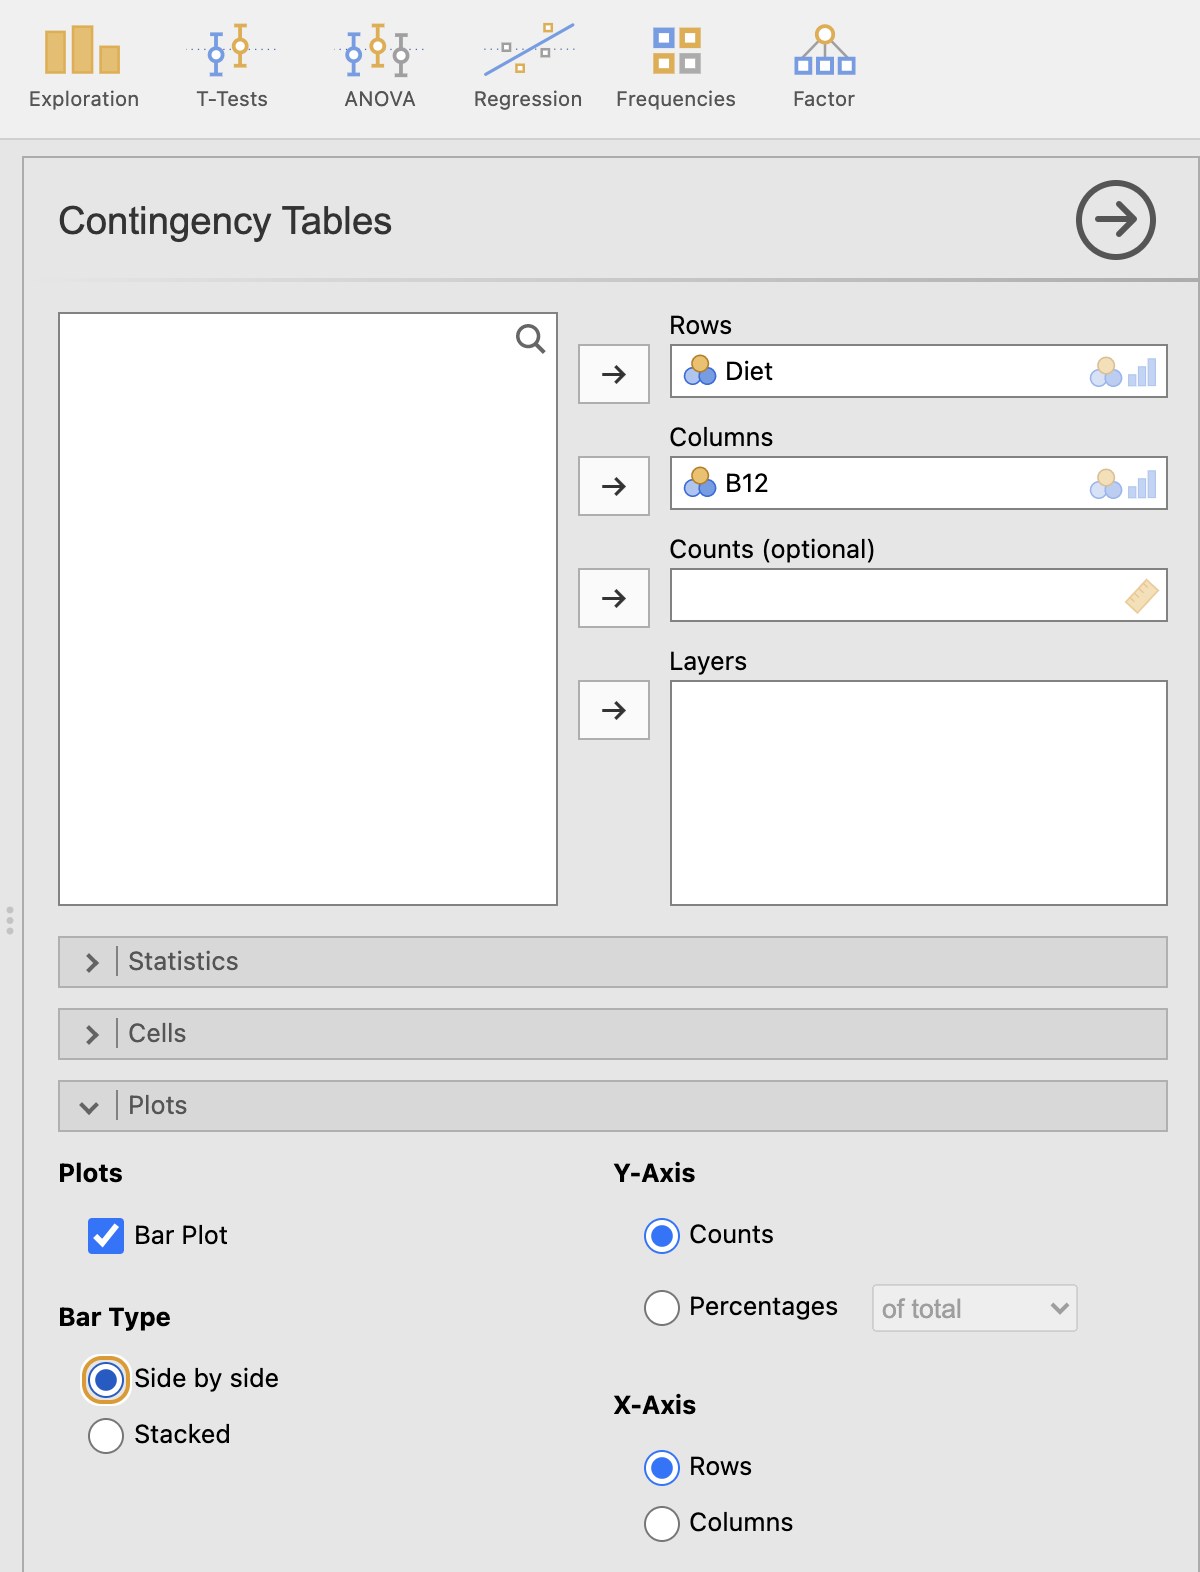
\includegraphics[width=0.5\linewidth]{jamoviImages/Chisq/B12-Barplot-Sidebyside} 

}

\caption{Adding the variables to create a side-by-side bar chart in jamovi}\label{fig:jamoviTwotFacePlant-Stacked-Barplot-new}
\end{figure}

\begin{enumerate}
\def\labelenumi{\arabic{enumi}.}
\setcounter{enumi}{4}
\tightlist
\item
  You can change the vertical axis to represent either counts or percentages by your selection under \textbf{Y-Axis}.
\item
  You can change which variables is on the horizontal axis by your selection under \textbf{X-Axis}.
  There are plenty of options, so feel free to experiment.
  A useful one is to use for the \textbf{Y-Axis} is \texttt{Percentages} with the \texttt{within\ rows} option.
\end{enumerate}

\begin{figure}[hbtp]

{\centering 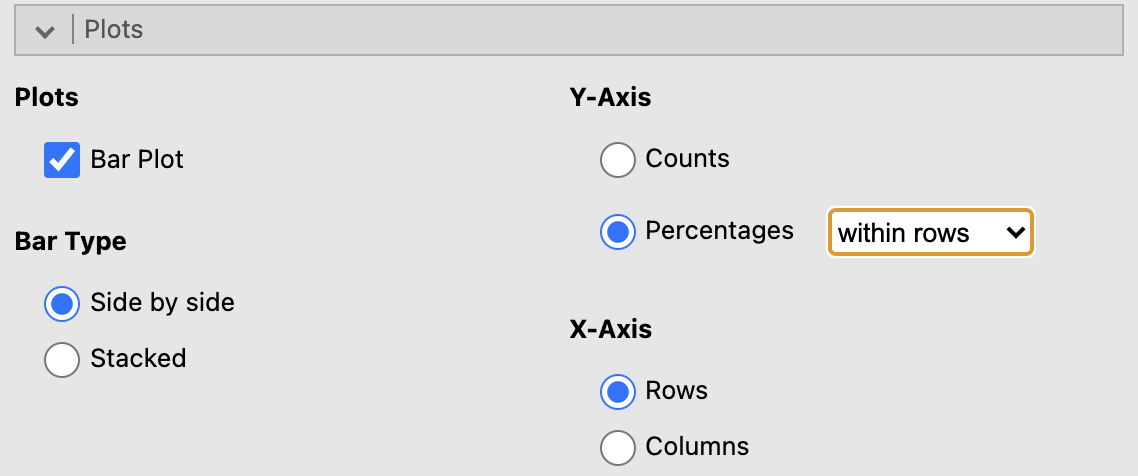
\includegraphics[width=0.5\linewidth]{jamoviImages/Chisq/B12-Barplot-Options} 

}

\caption{Adding the variables to create a side-by-side bar chart in jamovi}\label{fig:jamoviTwotFacePlant-Stacked-Barplot-options}
\end{figure}

\begin{enumerate}
\def\labelenumi{\arabic{enumi}.}
\setcounter{enumi}{5}
\tightlist
\item
  You will have your graph in the Output window.
\end{enumerate}

\section{Boxplots}\label{jamoviBoxplot}

For this section, the data introduced in Sect. \ref{jamoviLeanAngle} are used.

\begin{enumerate}
\def\labelenumi{\arabic{enumi}.}
\tightlist
\item
  \textbf{Use the jamovi menu:} select \textbf{Analyses\textgreater{} Exploration\textgreater{} Descriptives}.
\item
  \textbf{Add the variables}.
  Place the quantitative variable in the \emph{Variables} area, and the qualitative variable in the \textbf{Split by} area.
\item
  Then, click on the right-pointing arrow next to \textbf{Plots}, and in the \textbf{Box Plots} area select \texttt{Box\ plot}.
\item
  You will have your graph in the jamovi Output window.
\end{enumerate}

\begin{figure}[hbtp]

{\centering 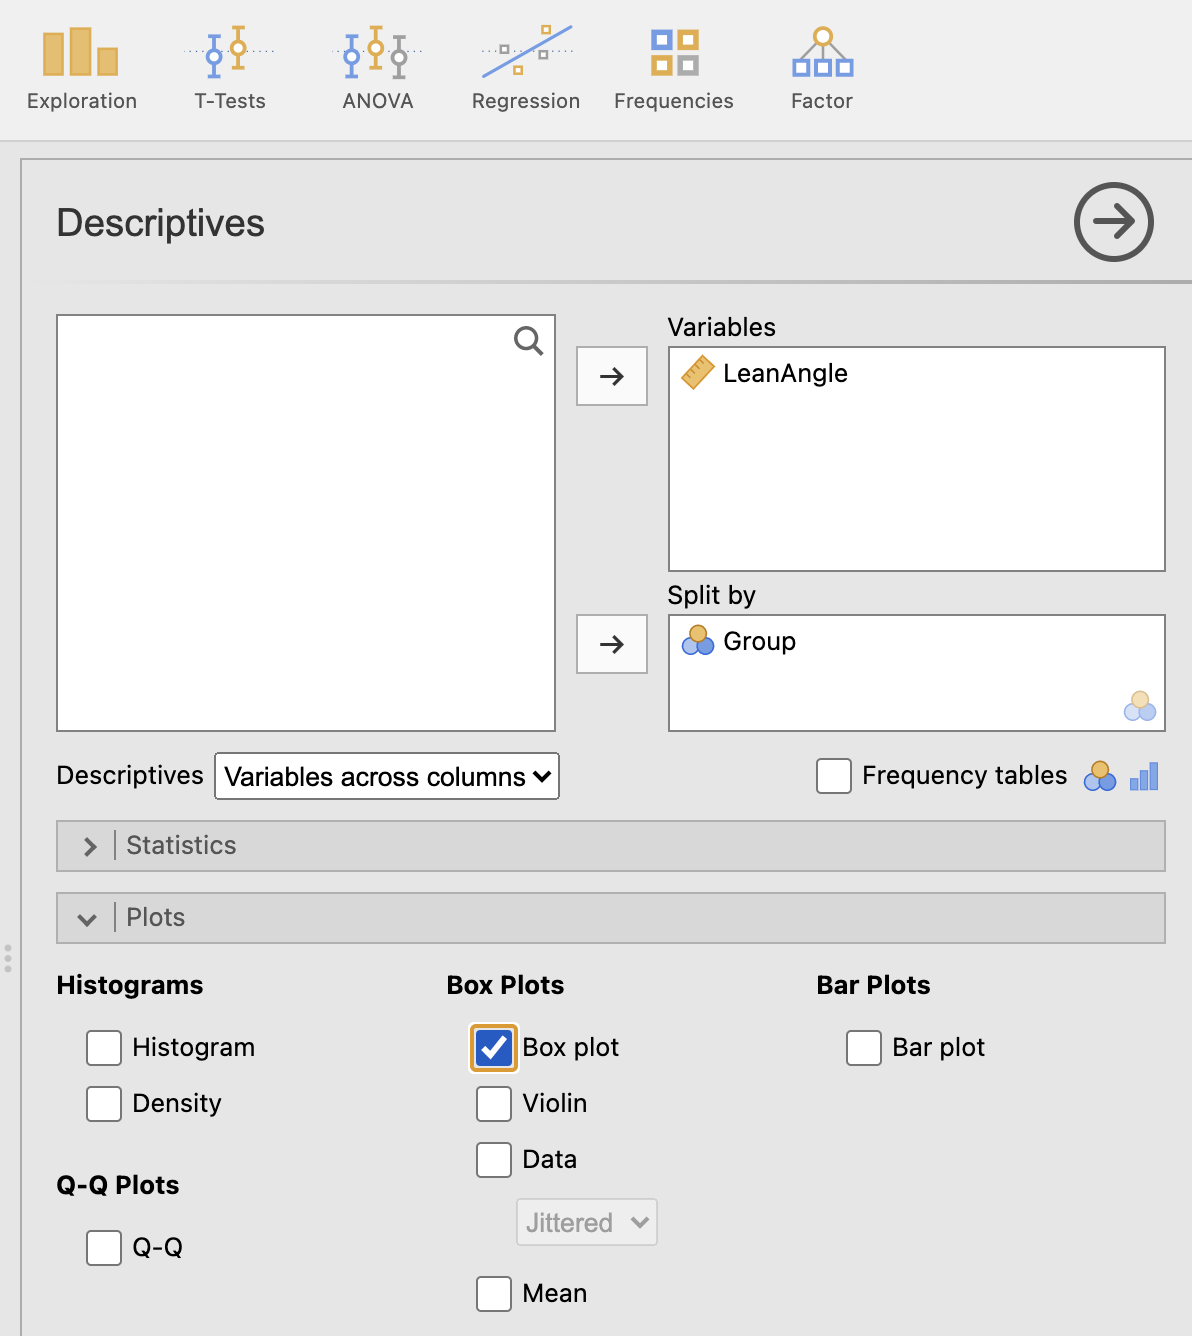
\includegraphics[width=0.5\linewidth]{jamoviImages/TwoInd/FacePlant-Boxplot} 

}

\caption{Selecting the variables for a boxplot}\label{fig:jamoviTwotFacePlant-Boxplot}
\end{figure}

\section{Error bar charts}\label{jamoviErrorbar}

Error bar charts are produced as part of the \emph{analysis}: see Chap. \ref{jamoviTwoSampleT}.

\section{Editing graphs}\label{jamoviEditGraphs}

At the time these notes were prepared, \emph{jamovi does not allow graphs to be edited} (but it is promised to be coming soon!).

\part{Using SPSS}\label{part-using-spss}

\chapter{SPSS: general information}\label{SPSSGeneral}

\begin{rmdobjectives}
\textbf{Topics} covered in this chapter:

\begin{itemize}
\tightlist
\item
  Tips for working with SPSS.
\end{itemize}
\end{rmdobjectives}

Before starting analysis with SPSS (\citeproc{ref-Software:SPSS}{IBM Corp 2016}), here are some \textbf{general tips}:

\begin{itemize}
\tightlist
\item
  In general, you cannot download a copy of SPSS for use at home (which you \emph{can} do with jamovi).
\item
  \emph{Except for graphs}, SPSS output should \textbf{not} be presented in reports or presentations.\\
  Instead, the information from SPSS output should be used to construct proper tables, or to produce proper conclusions.
\item
  SPSS has two worksheets sheets; \textbf{both} must be set up correctly (you can switch between the two worksheets by clicking on these at the bottom of the SPSS window):

  \begin{itemize}
  \tightlist
  \item
    The \textbf{Data View}, which contains the data.
  \item
    The \textbf{Variable View}, which contains information \emph{about} each variable.
  \end{itemize}
\item
  In SPSS (as with most statistical software), \emph{each row represents one unit of analysis} in the \textbf{Data View}.
\item
  In SPSS (as with most statistical software), \emph{each column represents one variable} in the \textbf{Data View}.
\item
  At the top of each column (but \textbf{not} in Row~1!) is the \emph{name} of the variable;
\item
  When setting up the \textbf{Variable View}, many columns can be filled in (Fig.~\ref{fig:SPSSVariables1}).
  These are the important columns to get right (the others aren't important for our purposes):

  \begin{itemize}
  \tightlist
  \item
    \textbf{Name}: A short description of the variable (with no spaces or punctuation!); for example \texttt{DiaBP}.
  \item
    \textbf{Type}: Usually \textbf{Numeric} (apart from \emph{names} which can be \textbf{String}).
  \item
    \textbf{Label}: A fuller description of the variable. This is what will appear in tables and graphs to describe the variable.
    For example \texttt{Diastolic\ blood\ pressure\ (in\ mm\ Hg)}.
  \item
    \textbf{Values}: For \emph{qualitative} variables only: tell SPSS what each number represents (for example, does a \texttt{1} represent females, or males?)
  \item
    \textbf{Measure}: \emph{This is important}:
    You must tell SPSS whether each variable is nominal, ordinal, or scale (i.e.~quantitative) by using the drop-down options.
  \end{itemize}
\item
  You can get help with using SPSS by:

  \begin{itemize}
  \tightlist
  \item
    Using \href{https://www.linkedin.com/learning/}{LinkedIn Learning}.
  \item
    Watching software screencasts on Canvas.
  \item
    Borrowing books in the library.
  \item
    Asking SCI110 staff, including using the Canvas \emph{Discussions}.
  \end{itemize}
\end{itemize}

\begin{figure}[hbtp]

{\centering 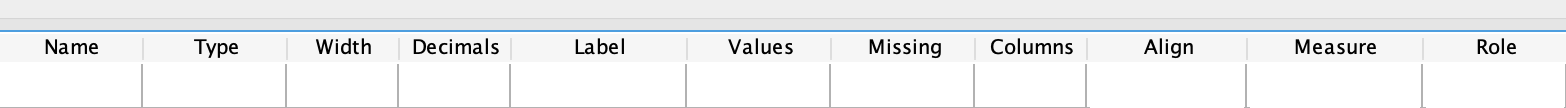
\includegraphics[width=1\linewidth]{SPSSImages/VarViewNames} 

}

\caption{Information that can be given for each variable in the Variable View window)}\label{fig:SPSSVariables1}
\end{figure}

\chapter{SPSS: inference for two odds or two proportions}\label{SPSSOR}

\begin{rmdobjectives}
\textbf{Topics} covered in this tutorial:

\begin{itemize}
\tightlist
\item
  How to use SPSS for comparing two odds (i.e., analysis using odds ratios).
\item
  How to use SPSS for comparing two proportions.
\end{itemize}
\end{rmdobjectives}

\section{Introduction}\label{SPSSB12Data}

\(\chi^2\) tests (`\emph{ki}-squared tests') are used to analyse data where each unit of analysis has \emph{two qualitative variables} measured (or observed) about it.
This type of data can be compiled into a two-way table of counts.

Consider data (\citeproc{ref-data:Gammon2012:B12}{Gammon et al. 2012}) \href{https://bookdown.org/pkaldunn/SRM-Textbook/AnalysisOddsRatio.html}{used in Exercise 31.16 of the textbook} (Table~\ref{tab:SPSSB12Data}).

\emph{Two qualitative variables} being measured on each individual:

\begin{enumerate}
\def\labelenumi{\arabic{enumi}.}
\tightlist
\item
  Whether the person is vegetarian (or not);
\item
  Whether the person is B12 deficient (or not);
\end{enumerate}

So SPSS will have \emph{two columns}: one for each variable.

\begin{rmddatafile}
The data file (\texttt{B12-Long.sav}) can be downloaded in Sect. \ref{DataFiles}.

You can download the data, and follow the instructions.
\end{rmddatafile}

\begin{table}
\centering
\caption{\label{tab:SPSSB12Data}The number of vegetarian and non-vegetarian women who are (and are not) B12 deficient}
\centering
\fontsize{10}{12}\selectfont
\begin{tabular}[t]{lrr>{}r}
\toprule
\textbf{ } & \textbf{B12 deficient} & \textbf{Not B12 deficient} & \textbf{Total}\\
\midrule
Vegetarians & 8 & 26 & \textbf{34}\\
Non-vegetarians & 8 & 82 & \textbf{90}\\
\midrule
\textbf{Total} & \textbf{16} & \textbf{108} & \textbf{\textbf{124}}\\
\bottomrule
\end{tabular}
\end{table}

\section{Data entry}\label{SPSSChiSquareDataEntry}

In the SPSS \textbf{Variable View}:

\begin{itemize}
\tightlist
\item
  \textbf{Diet}: \texttt{1} means `Vegetarian' (i.e.~in Row~1 of the data table),
  and \texttt{2} means `Non-vegetarian' (i.e.~in Row~2 of the data table).
\item
  \textbf{B12}: \texttt{1} means `B12 deficient' (i.e.~in Column~1 of the data table),
  and \texttt{2} means `\emph{Not} B12 deficient' (i.e.~in Column~2 of the data table).
\end{itemize}

See Fig. \ref{fig:SPSSVariables1}.

The usual approach for data entry used by SPSS is that \emph{each row represents one unit of analysis}.
That means that there will be \(124\) rows of data: one for each person (unit of analysis).

In SPSS, the data are entered as shown in Fig.~\ref{fig:SPSSVariables1a}, but there would be \(124\)~rows.

\begin{figure}[hbtp]

{\centering 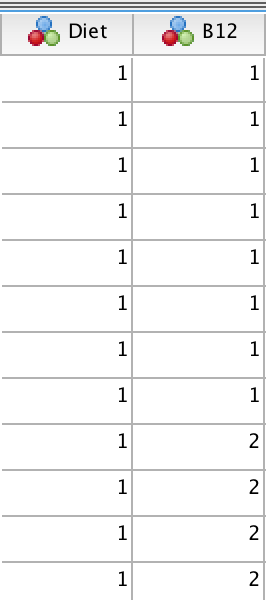
\includegraphics[width=0.2\linewidth]{SPSSImages/Chisq/B12-Data-Long} 

}

\caption{Data entered into SPSS}\label{fig:SPSSVariables1a}
\end{figure}

The \textbf{Variable View} would describe these two variables; see Fig.~\ref{fig:SPSSVariables2}.

\begin{figure}[hbtp]

{\centering 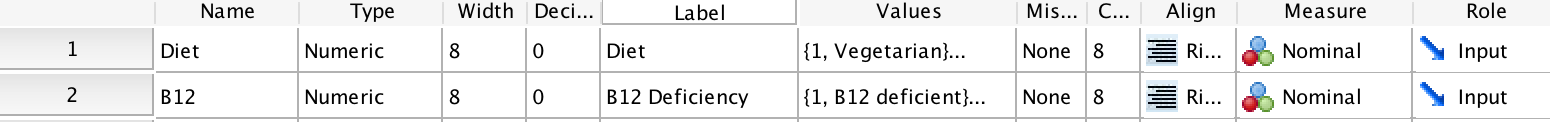
\includegraphics[width=1\linewidth]{SPSSImages/Chisq/B12-VarView-Long} 

}

\caption{Describing the variable in the Variable View window}\label{fig:SPSSVariables2}
\end{figure}

\section{Analysis}\label{SPSSChiSquareAnalysis}

Once the data are entered, we can begin analysis:

\begin{enumerate}
\def\labelenumi{\arabic{enumi}.}
\item
  \textbf{Use the menu:} select \textbf{Analyze\textgreater{} Descriptive Statistics\textgreater{} Crosstabs\ldots{}}
\item
  \textbf{Select the variables}, dragging them from the left panel to the \textbf{Row(s)} and \textbf{Column(s)} areas as appropriate.
  In Table~\ref{tab:SPSSB12Data}, \textbf{Diet} is in the rows of the table, for example.
  See Fig.~\ref{fig:SPSSB12VariablesIn}.
\end{enumerate}

\begin{figure}[hbtp]

{\centering 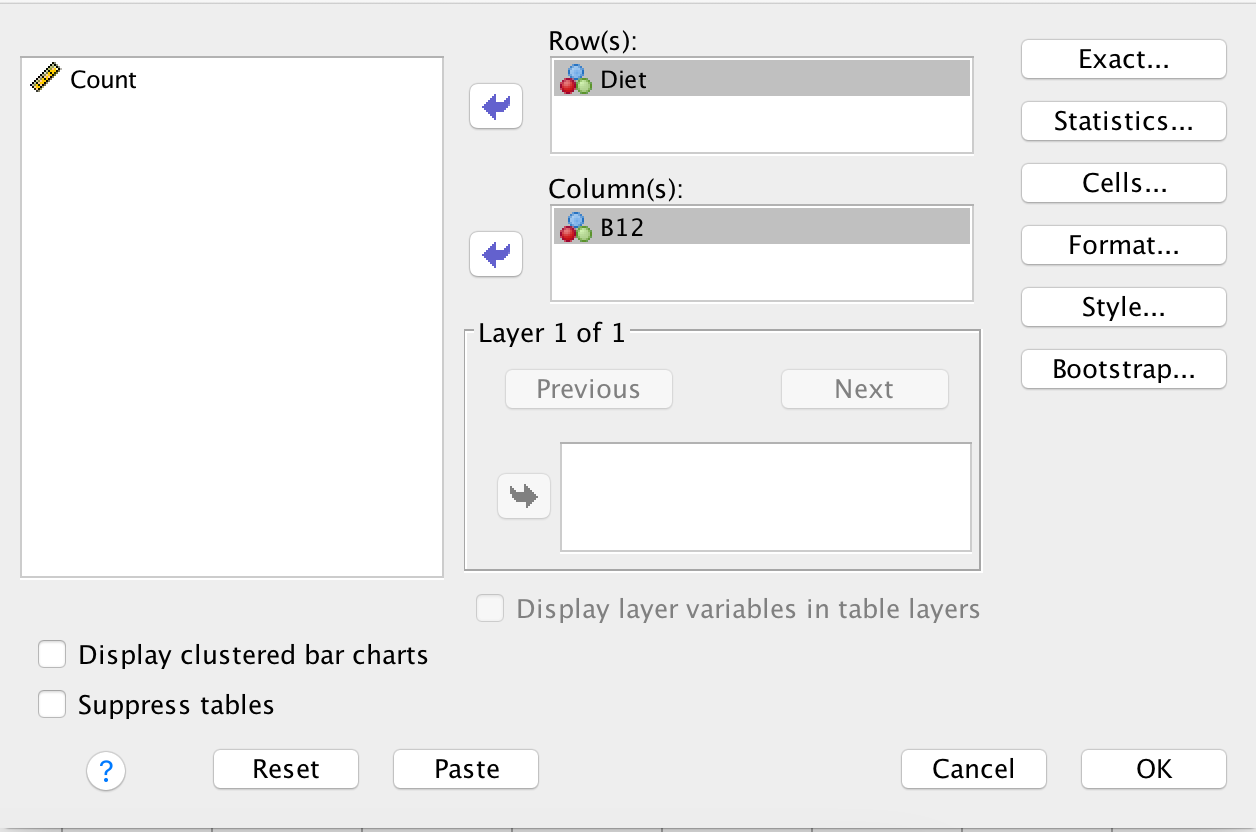
\includegraphics[width=0.85\linewidth]{SPSSImages/Chisq/B12-Analysis} 

}

\caption{Add the variables}\label{fig:SPSSB12VariablesIn}
\end{figure}

\begin{enumerate}
\def\labelenumi{\arabic{enumi}.}
\setcounter{enumi}{2}
\tightlist
\item
  \textbf{Select the analysis options.}
  Click the \textbf{Statistics\ldots{}} button, and then (Fig.~\ref{fig:SPSSB12Analysis}):

  \begin{itemize}
  \tightlist
  \item
    Select the \textbf{Chi-square}: to produce information for the hypothesis test.
  \item
    Select the \textbf{Risk} option: to produce a CI for the odds ratio.
  \end{itemize}
\item
  Press \textbf{Continue}, and then press \textbf{OK}.
  You will have your output in the SPSS Output window.
\end{enumerate}

\begin{figure}[hbtp]

{\centering 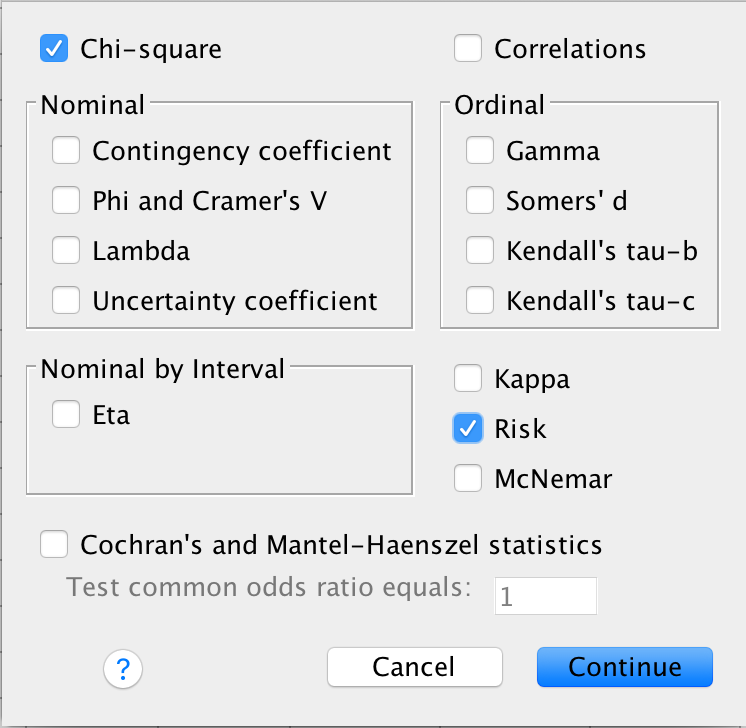
\includegraphics[width=0.55\linewidth]{SPSSImages/Chisq/B12-Analysis-Ticks} 

}

\caption{Select the options}\label{fig:SPSSB12Analysis}
\end{figure}

\section{Numerical summaries}\label{SPSSChiSquareNumericalSummaries}

\textbf{Percentages} can be obtained from \textbf{Analyze\textgreater{} Descriptive Statistics\textgreater{} Crosstabs\ldots{}}
In the window that appears, select \textbf{Cells\ldots{}} and then select \textbf{Percentages} as \textbf{Row}, as \textbf{Column}, or even as both if you wish.

\emph{Odds} are computed as part of the inference output from Sect.~\ref{SPSSChiSquareAnalysis}.

\chapter{SPSS: inference about the difference between two means}\label{SPSSTwoSampleT}

\begin{rmdobjectives}
\textbf{Topics} covered in this tutorial:

\begin{itemize}
\tightlist
\item
  Learn how to use SPSS for comparing two means.
\end{itemize}
\end{rmdobjectives}

\section{Introduction}\label{SPSSLeanAngle}

Two independent sample \(t\)-tests are used to compare the means of two separate groups.

Consider the face-plant data (\citeproc{ref-data:Wojcik:ForwardFall}{Wojcik et al. 1999}) \href{https://bookdown.org/pkaldunn/SRM-Textbook/AnalysisTwoMeans.html}{used in Exercise~30.11 of the textbook} (Table~\ref{tab:SPSSFacePlant}).

\begin{table}
\centering
\caption{\label{tab:SPSSFacePlant}Lean-forward angles for older and younger women}
\centering
\fontsize{10}{12}\selectfont
\begin{tabular}[t]{ccc}
\toprule
\multicolumn{2}{c}{\textbf{Younger women }} & \multicolumn{1}{c}{\textbf{Older women }} \\
\cmidrule(l{3pt}r{3pt}){1-2} \cmidrule(l{3pt}r{3pt}){3-3}
29 & 34 & 18\\
32 & 27 & 15\\
34 & 32 & 23\\
31 & 28 & 13\\
33 & 27 & 12\\
\bottomrule
\end{tabular}
\end{table}

\begin{rmddatafile}
The data file (\texttt{forwardfall.sav}) can be downloaded in Sect. \ref{DataFiles}.

You can download the data, and follow the instructions.
\end{rmddatafile}

\section{Data entry}\label{SPSSTwoSampleAnalysisDataEntry}

In the \textbf{Data View}, each row represents a unit of analysis (in this case, a person), as is usual in SPSS.

Each unit of analysis gets two variables recorded on it: one is quantitative (\texttt{LeanAngle}), and one is qualitative (\texttt{Group}).
So there are two columns in the \textbf{Data View}, one for each variable.

The order doesn't matter, but here the quantitative variable is listed first (the lean-forward angle), and then the qualitative variable (the age group).

The \textbf{Variable View} needs to be set up correctly too (Fig.~\ref{fig:SPSSFacePlantVariablesIn}).
For example, all variables should be given a descriptive label.
The quantitative variable (here, \texttt{LeanAngle}) should be declared as \textbf{Scale} in the \textbf{Measure} column.
The qualitative variable (here, \texttt{Group}) should be declared as \textbf{Nominal} in the \textbf{Measure} column (Fig.~\ref{fig:SPSSFacePlantVariablesVV}).

\begin{figure}[hbtp]

{\centering 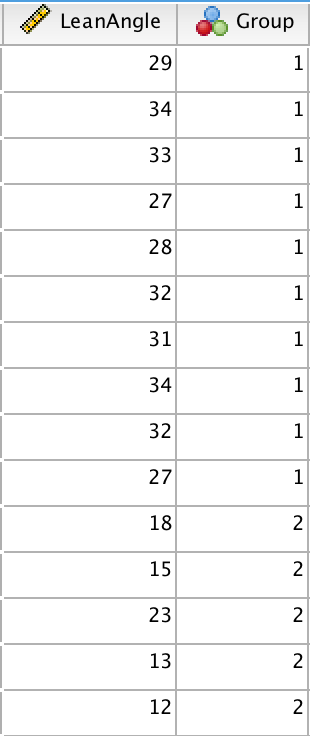
\includegraphics[width=0.3\linewidth]{SPSSImages/FacePlant-Data} 

}

\caption{The data in the Data View}\label{fig:SPSSFacePlantVariablesIn}
\end{figure}

\begin{figure}[hbtp]

{\centering 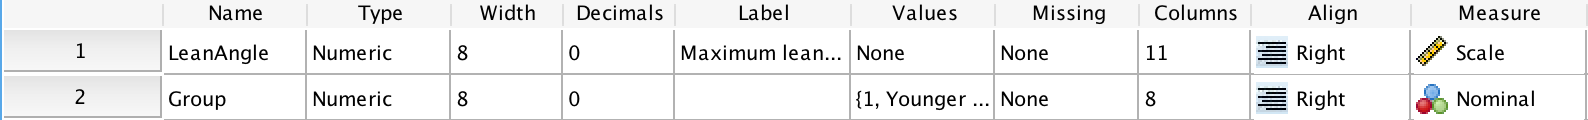
\includegraphics[width=1\linewidth]{SPSSImages/FacePlant-VarView} 

}

\caption{The Variable View}\label{fig:SPSSFacePlantVariablesVV}
\end{figure}

The two age groups are defined so that a \texttt{1} represents younger women, and a \texttt{2} represents older women.
Since this is arbitrary, we tell SPSS this by setting the \textbf{Values} in the \textbf{Variable View} (Fig.~\ref{fig:SPSSFacePlantVariablesLevels}).

\begin{figure}[hbtp]

{\centering 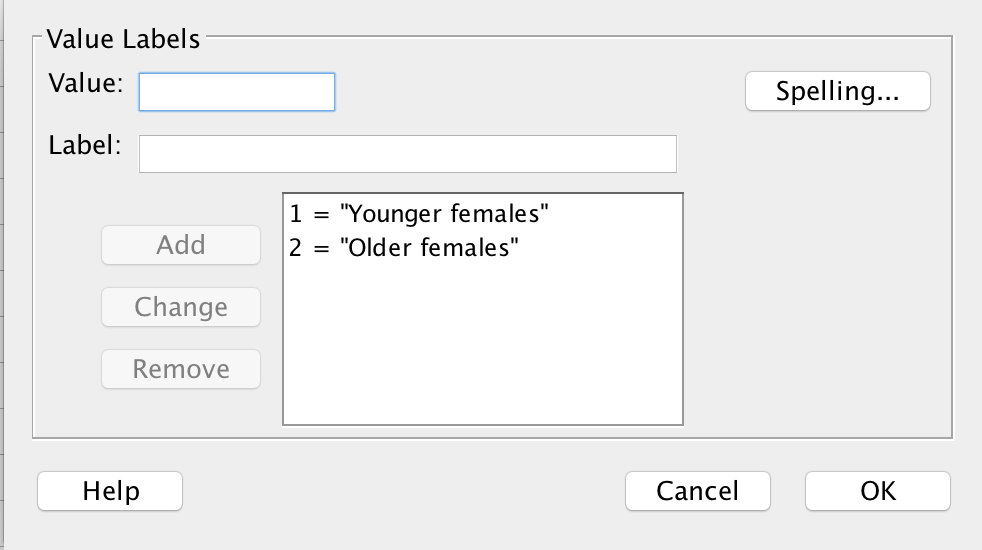
\includegraphics[width=0.85\linewidth]{SPSSImages/FacePlant-Levels} 

}

\caption{Defining the levels (Values) for the age group, in the Variable View}\label{fig:SPSSFacePlantVariablesLevels}
\end{figure}

\section{Analysis}\label{SPSSTwoSampleAnalysis}

\begin{enumerate}
\def\labelenumi{\arabic{enumi}.}
\tightlist
\item
  \textbf{Use the SPSS menu}: select \textbf{Analyze\textgreater{} Compare Means\textgreater{} Independent Samples T Test\ldots{}}
\item
  \textbf{Select the Variables}.
  The \textbf{Test Variable} is the quantitative variable (here, \texttt{LeanAngle}), and the \textbf{Grouping Variable} is the qualitative variable (here, `\texttt{Group}); see Fig.~\ref{fig:SPSSFacePlantVarsIn}.
\end{enumerate}

\begin{figure}[hbtp]

{\centering 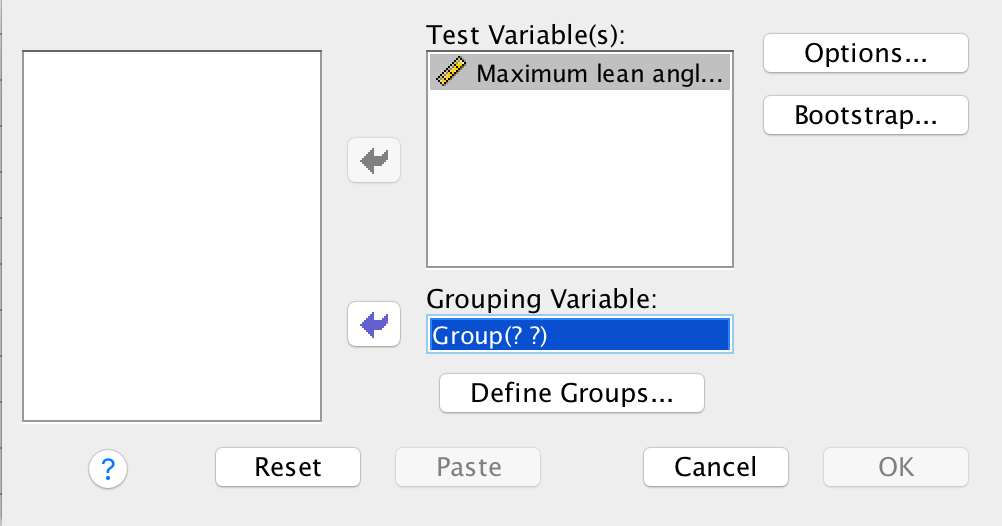
\includegraphics[width=0.85\linewidth]{SPSSImages/FacePlant-Variables} 

}

\caption{Entering the variables}\label{fig:SPSSFacePlantVarsIn}
\end{figure}

\begin{enumerate}
\def\labelenumi{\arabic{enumi}.}
\setcounter{enumi}{2}
\tightlist
\item
  \textbf{Define the groups to compare}.
  Click the button \textbf{Define Groups\ldots{}} and enter the numbers that are being used to represent the two groups to be compared.
  In this example, the two groups are given the values \texttt{1} and \texttt{2} in the \textbf{Data View}, so we enter these.
\item
  Click the \textbf{Continue} button, then \textbf{OK}.
  You will have your output in the SPSS Output window.
\end{enumerate}

\begin{figure}[hbtp]

{\centering 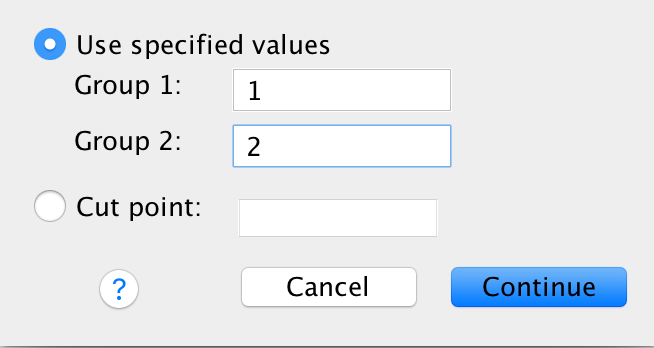
\includegraphics[width=0.5\linewidth]{SPSSImages/FacePlant-Groups} 

}

\caption{Teling SPSS which groups to compare}\label{fig:SPSSFacePlantVarsInwegcucwg}
\end{figure}

\section{Numerical summaries}\label{SPSSTwoSampleAnalysisNumericalSummaries}

The \emph{mean}, \emph{median}, \emph{standard deviation} and \emph{standard error} are produced as part of the output from the \(t\)-test analysis step above.

The \emph{mean} and \emph{standard error} for the \emph{difference} is obtained from the \(t\)-test output too; see Sect.~\ref{SPSSTwoSampleAnalysis}.

\chapter{SPSS: graphs}\label{SPSSGraphs}

\begin{rmdobjectives}
\textbf{Topics} covered in this tutorial:

\begin{itemize}
\tightlist
\item
  Creating graphs in SPSS.
\end{itemize}
\end{rmdobjectives}

\begin{rmddatafile}
The data files used in this section can be downloaded in Sect. \ref{DataFiles}.

You can download the data, and follow the instructions.
\end{rmddatafile}

Graphs in SPSS are generally produced using the \textbf{Graphs} menu, and then selecting \textbf{Chart Builder\ldots{}}

After making this selection, you usually get a warning (Fig.~\ref{fig:SPSSGraphWarning})).
It is reminding you that it is \textbf{really important} that your have declared the \textbf{Measure} correctly for each variable
in the \textbf{Variable View} (that is, correctly declared each variable as \textbf{Nominal}, \textbf{Ordinal} or \textbf{Scale}); see Sect.~\ref{SPSSGeneral}.

Provided you have done so, you can press \textbf{OK}.

\begin{figure}[hbtp]

{\centering 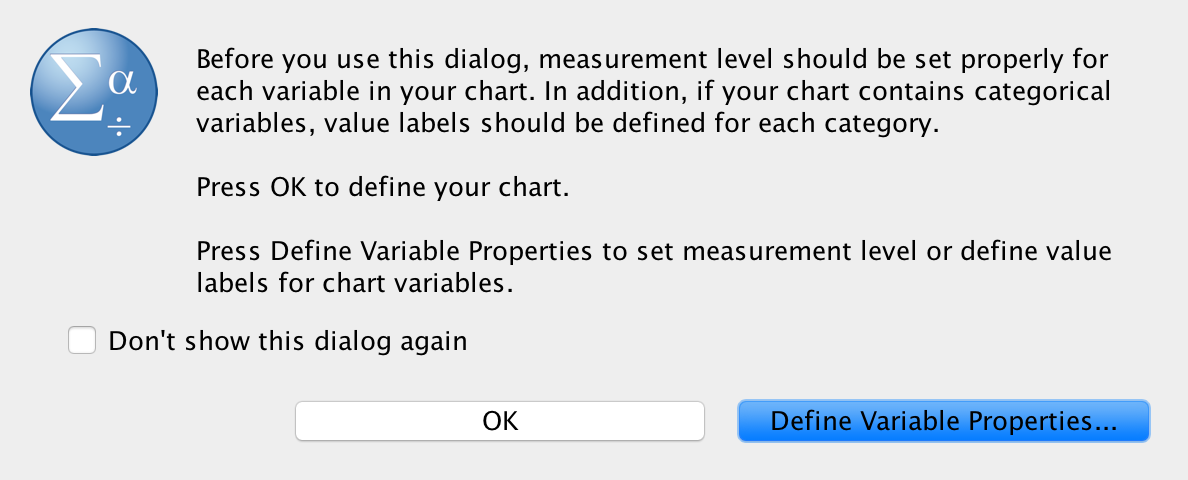
\includegraphics[width=0.85\linewidth]{SPSSImages/Graphics-Warning} 

}

\caption{The warning after selecting Graphs}\label{fig:SPSSGraphWarning}
\end{figure}

\begin{rmdimportant}
The graphs produced by default in SPSS are usually an inconvenient size for copying-and-pasting into Word, PowewrPoint, and other places.
We now explain the easy solution.
\end{rmdimportant}

When graphs are created in SPSS using the \textbf{Chart Builder}, the window shown in Fig.~\ref{fig:SPSSChartBuilder} initially appears.
Select the \textbf{Options} item from the right-hand side of this window.

\begin{figure}[hbtp]

{\centering 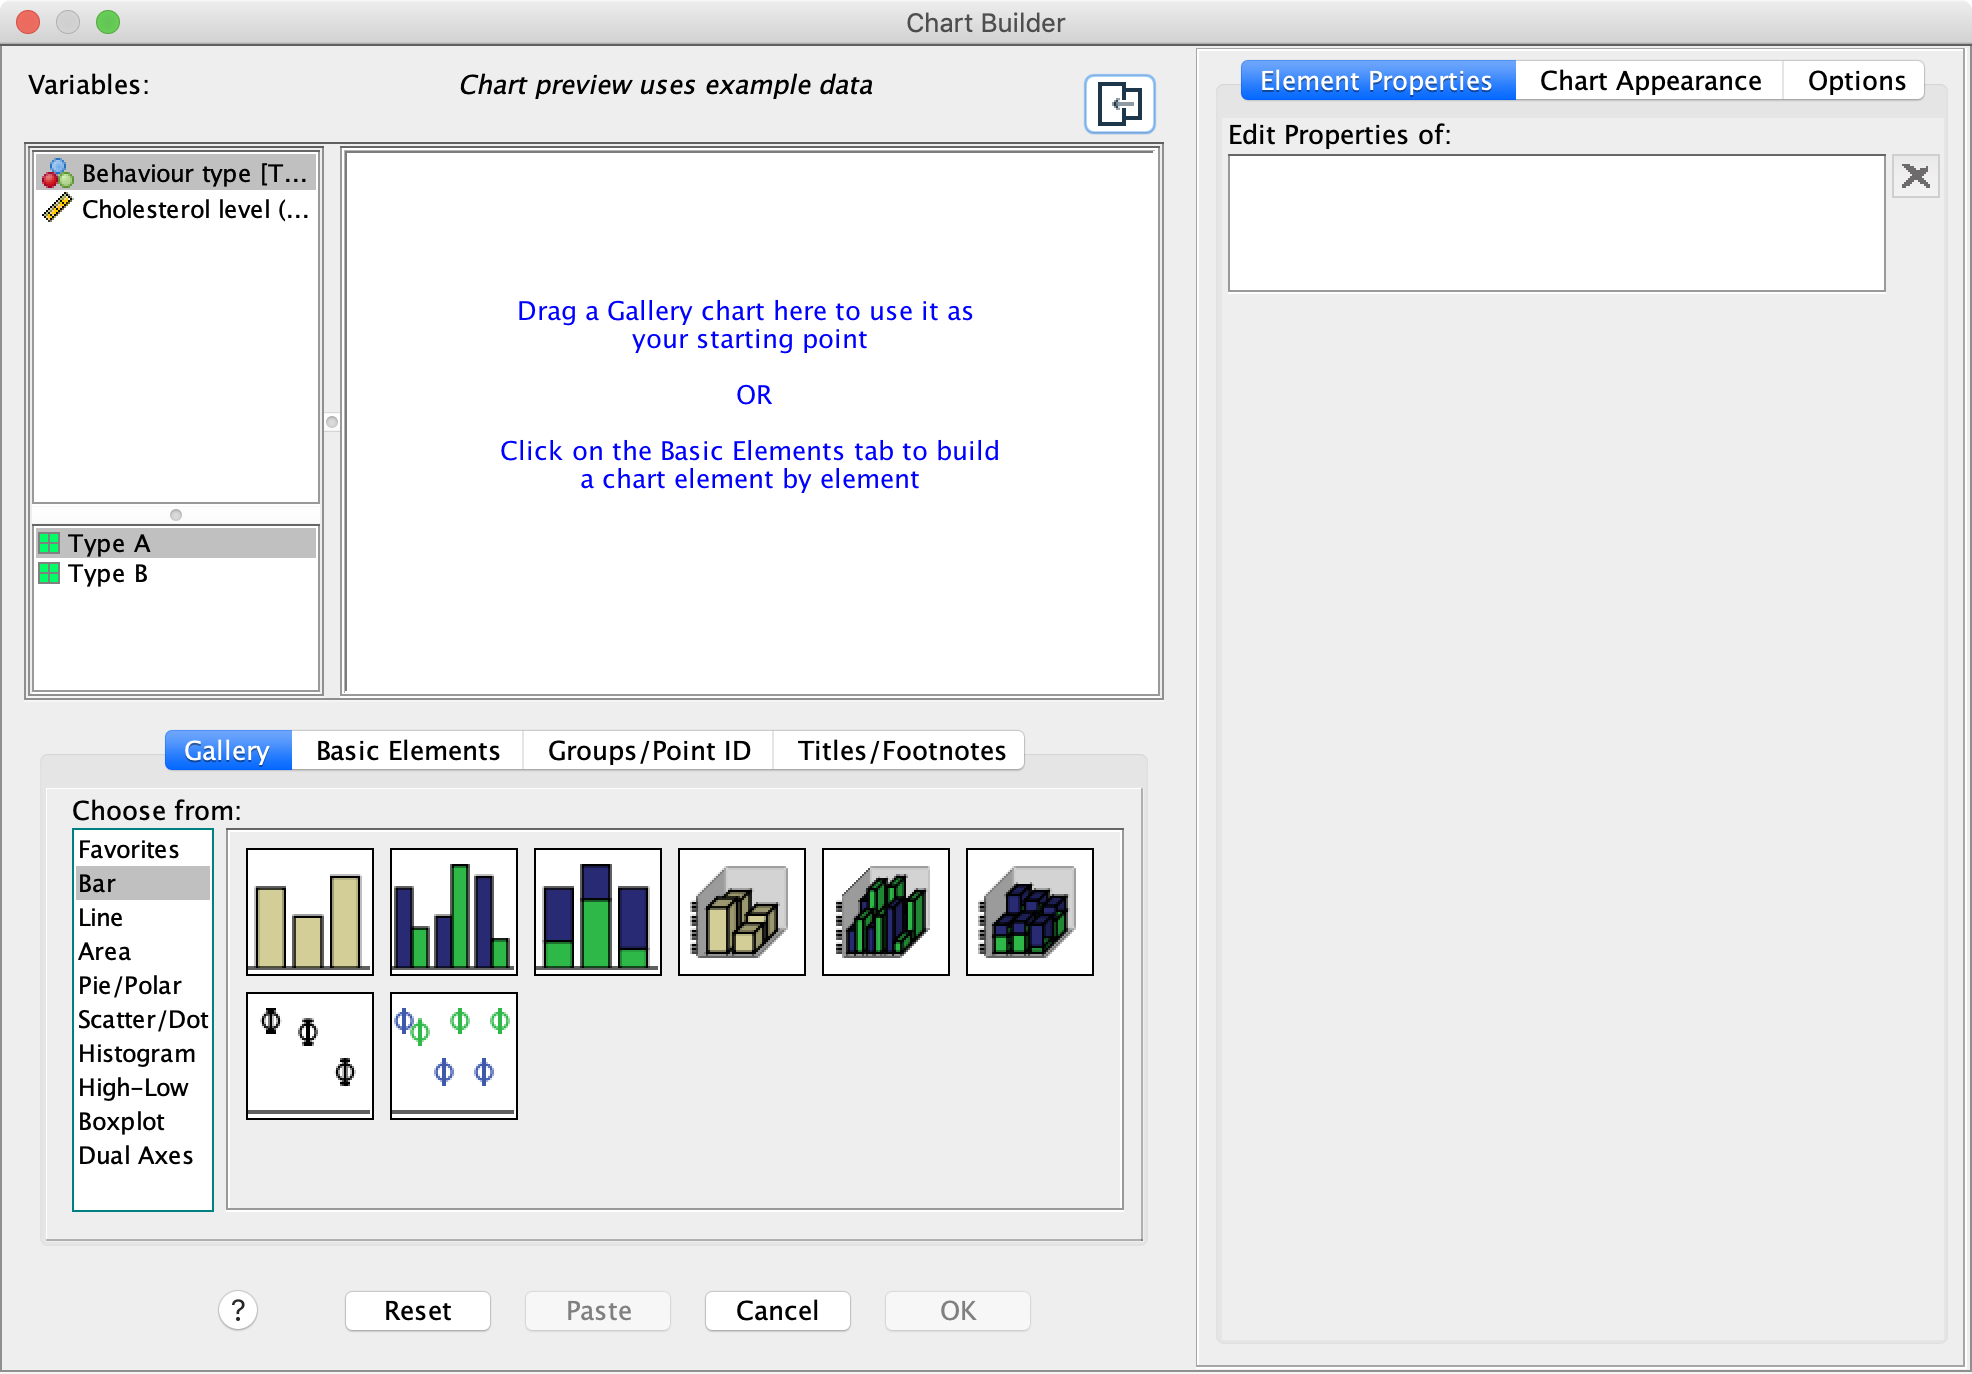
\includegraphics[width=0.85\linewidth]{SPSSImages/ChartBuilder} 

}

\caption{The Chart Builder window}\label{fig:SPSSChartBuilder}
\end{figure}

Then, change the \textbf{Chart size} to (say) 60\% or a similar value (Fig.~\ref{fig:SPSSChartBuilderOptions}).
Now, when you copy-and-paste the graph, the sizing will be more appropriate.

\begin{figure}[hbtp]

{\centering 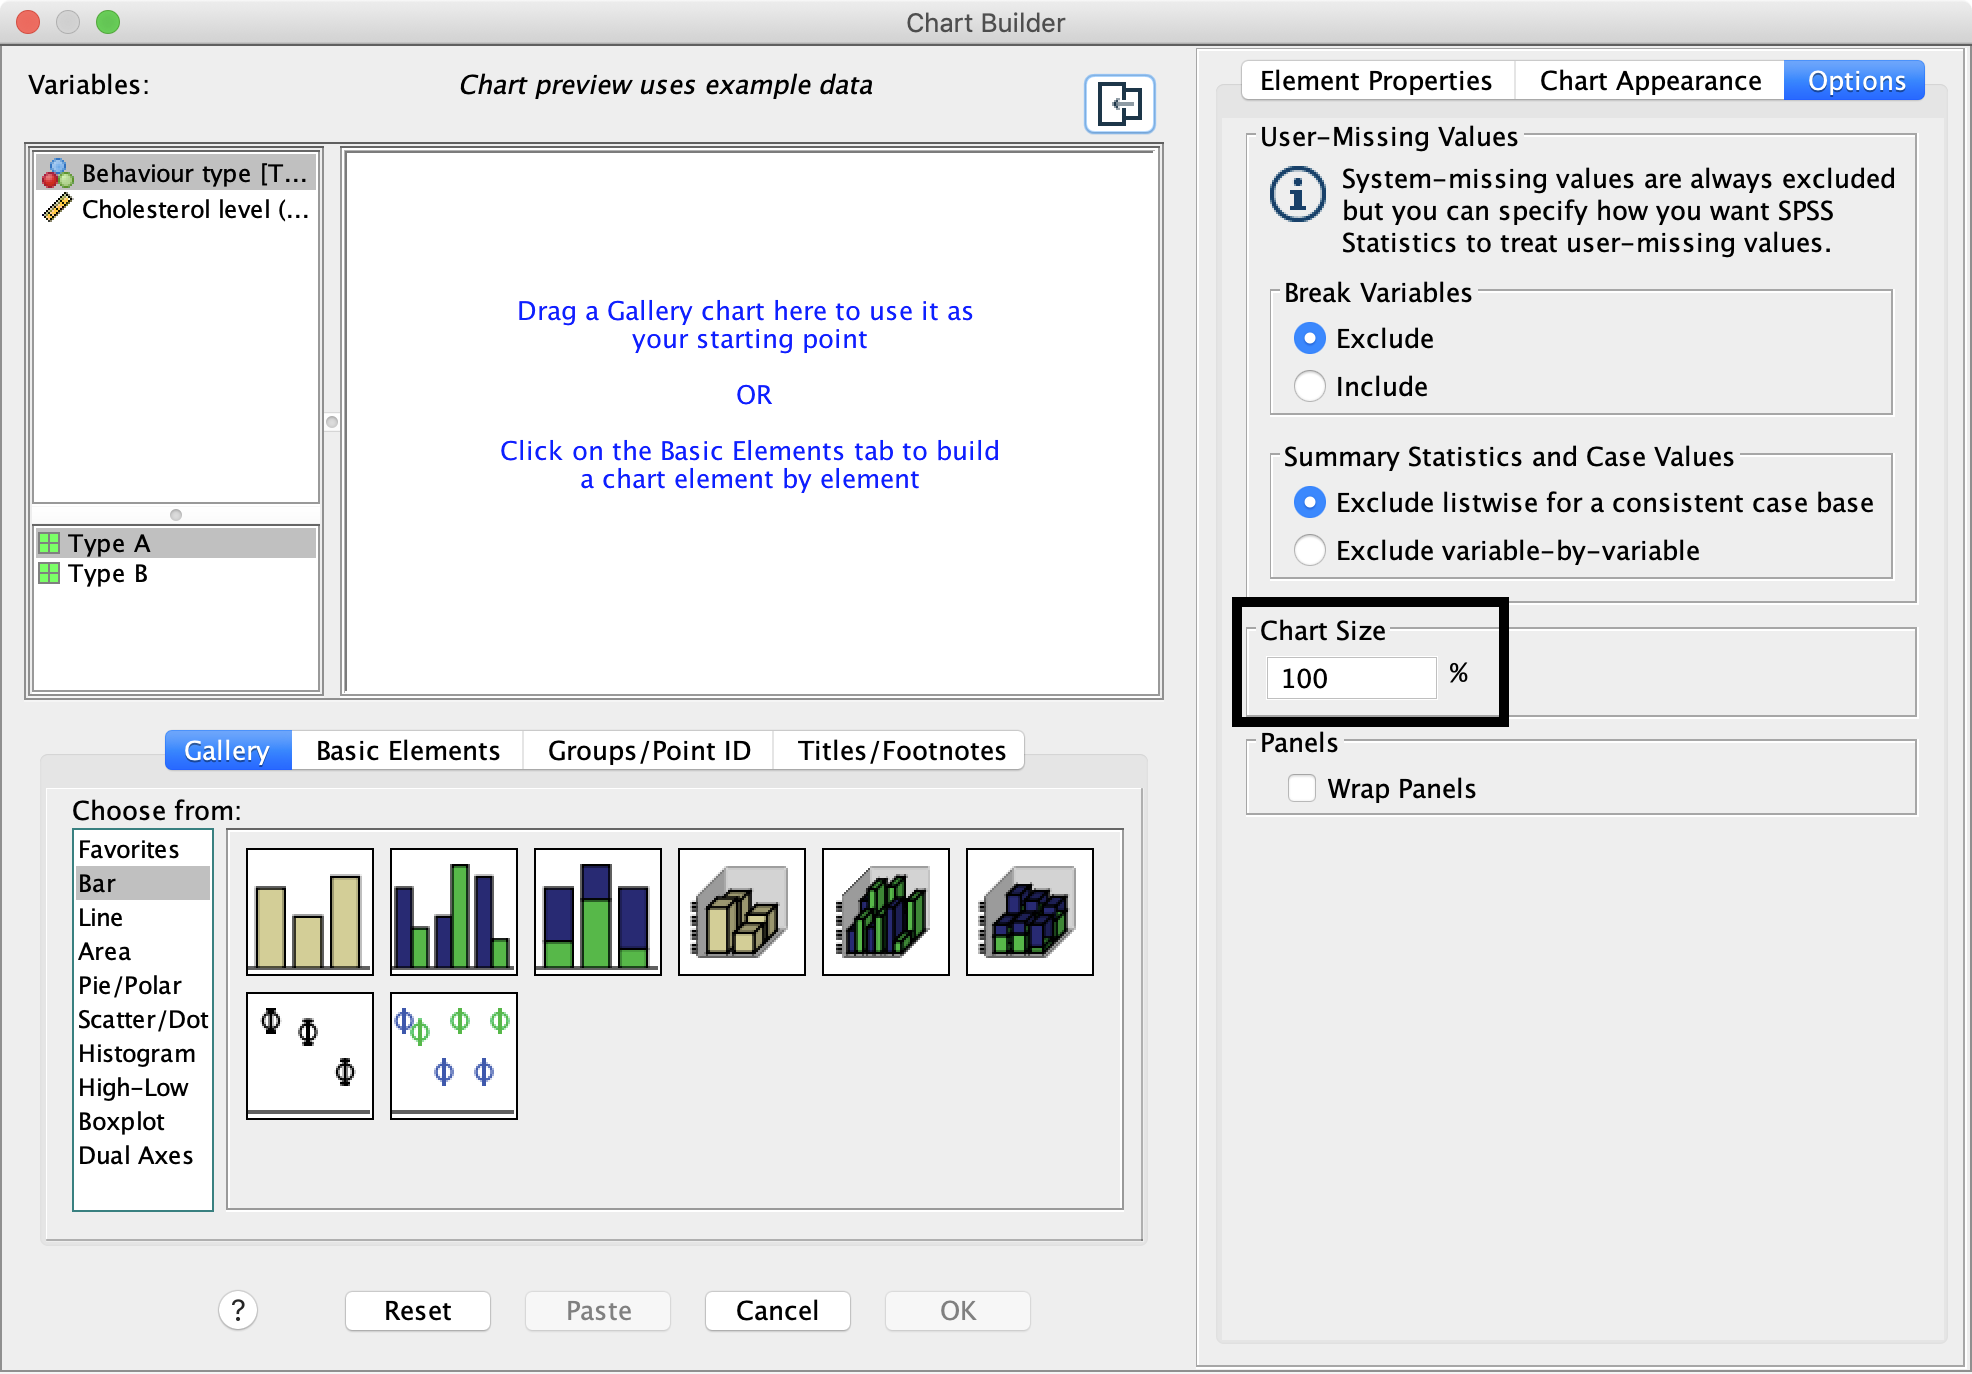
\includegraphics[width=0.85\linewidth]{SPSSImages/ChartBuilder-Options-Size} 

}

\caption{The warning after selecting Graphs}\label{fig:SPSSChartBuilderOptions}
\end{figure}

\section{Side-by-side bar charts}\label{SPSSSideBySide}

For this section, the data introduced in Sect. \ref{SPSSB12Data} are used.

\begin{enumerate}
\def\labelenumi{\arabic{enumi}.}
\tightlist
\item
  \textbf{Use the SPSS menu:} select \textbf{Graphs\textgreater{} Chart Builder\ldots{}}
\item
  \textbf{Select the type of plot}.
  Select \textbf{Bar} from the Gallery, then select the \textbf{second} template from the top row, and drag it to the canvas.
\end{enumerate}

\begin{figure}[hbtp]

{\centering 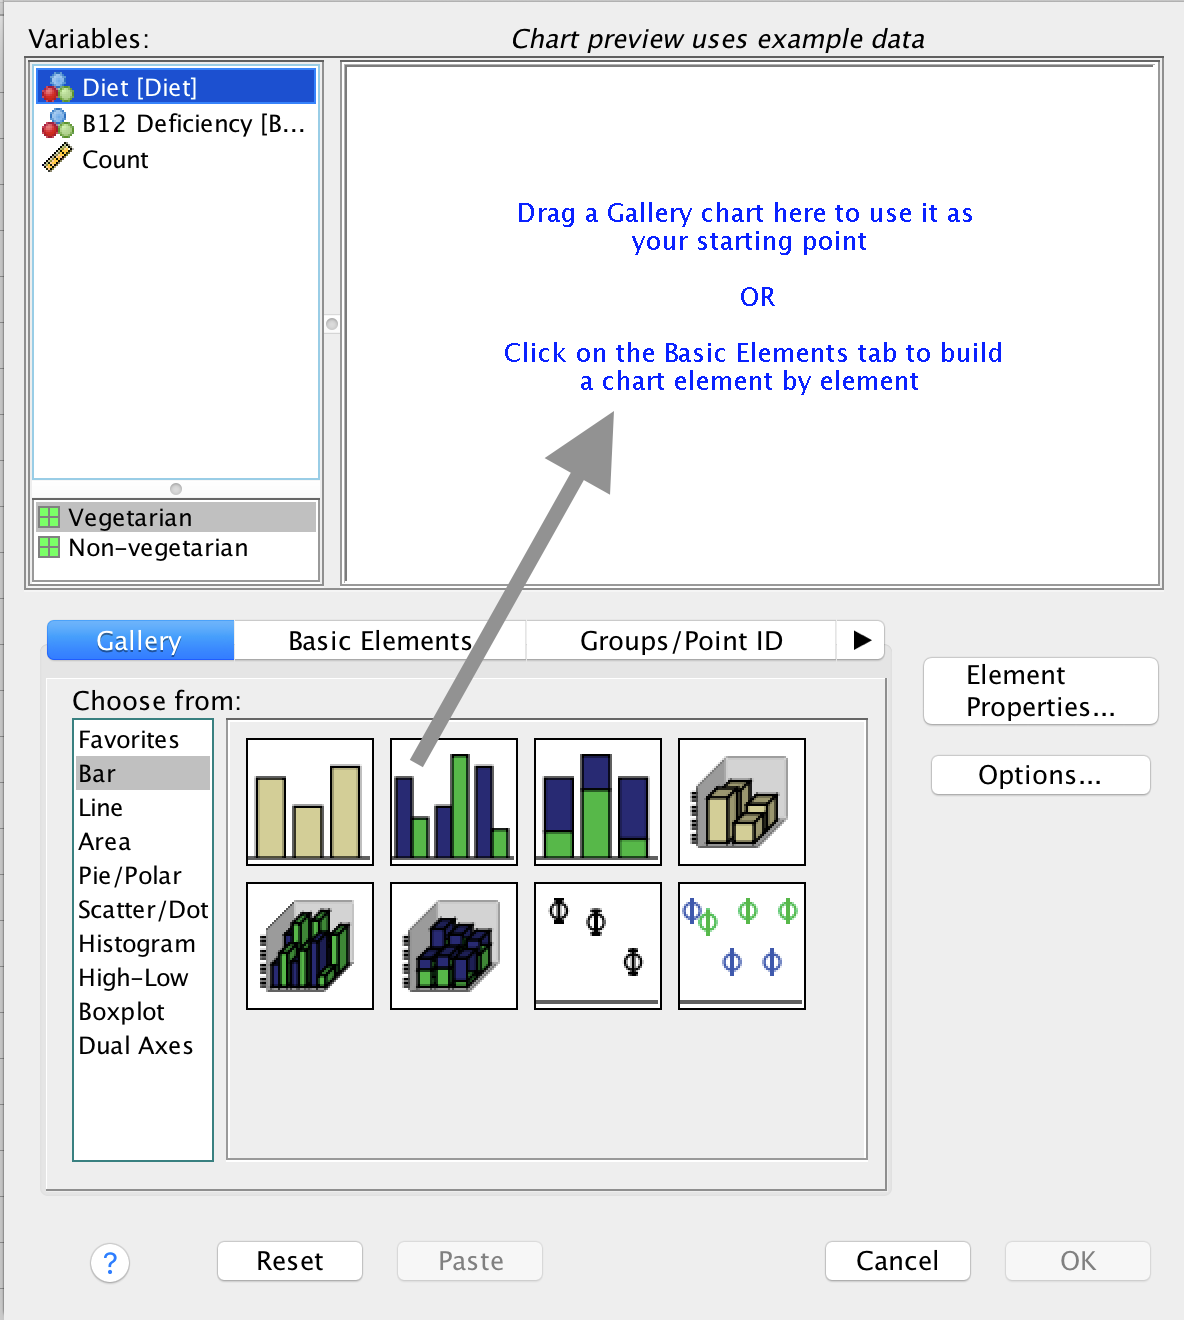
\includegraphics[width=0.85\linewidth]{SPSSImages/Chisq/B12-GraphicsWindow-SbS} 

}

\caption{Selecting a side-by-side bar chart}\label{fig:SPSSGraphSbS}
\end{figure}

\begin{enumerate}
\def\labelenumi{\arabic{enumi}.}
\setcounter{enumi}{2}
\tightlist
\item
  \textbf{Add the variables}.
  Drag one qualitative variable to the bottom (left-to-right) axis; this can often be seen as the explanatory variable.
  Drag the other to the top right (where it says, cryptically, \textbf{Cluster on X: set color}); see Fig.~\ref{fig:SPSSGraphSbSAddVars}).
\item
  Press \textbf{OK}.
  You will have your graph in the SPSS Output window.
\end{enumerate}

\begin{figure}[hbtp]

{\centering 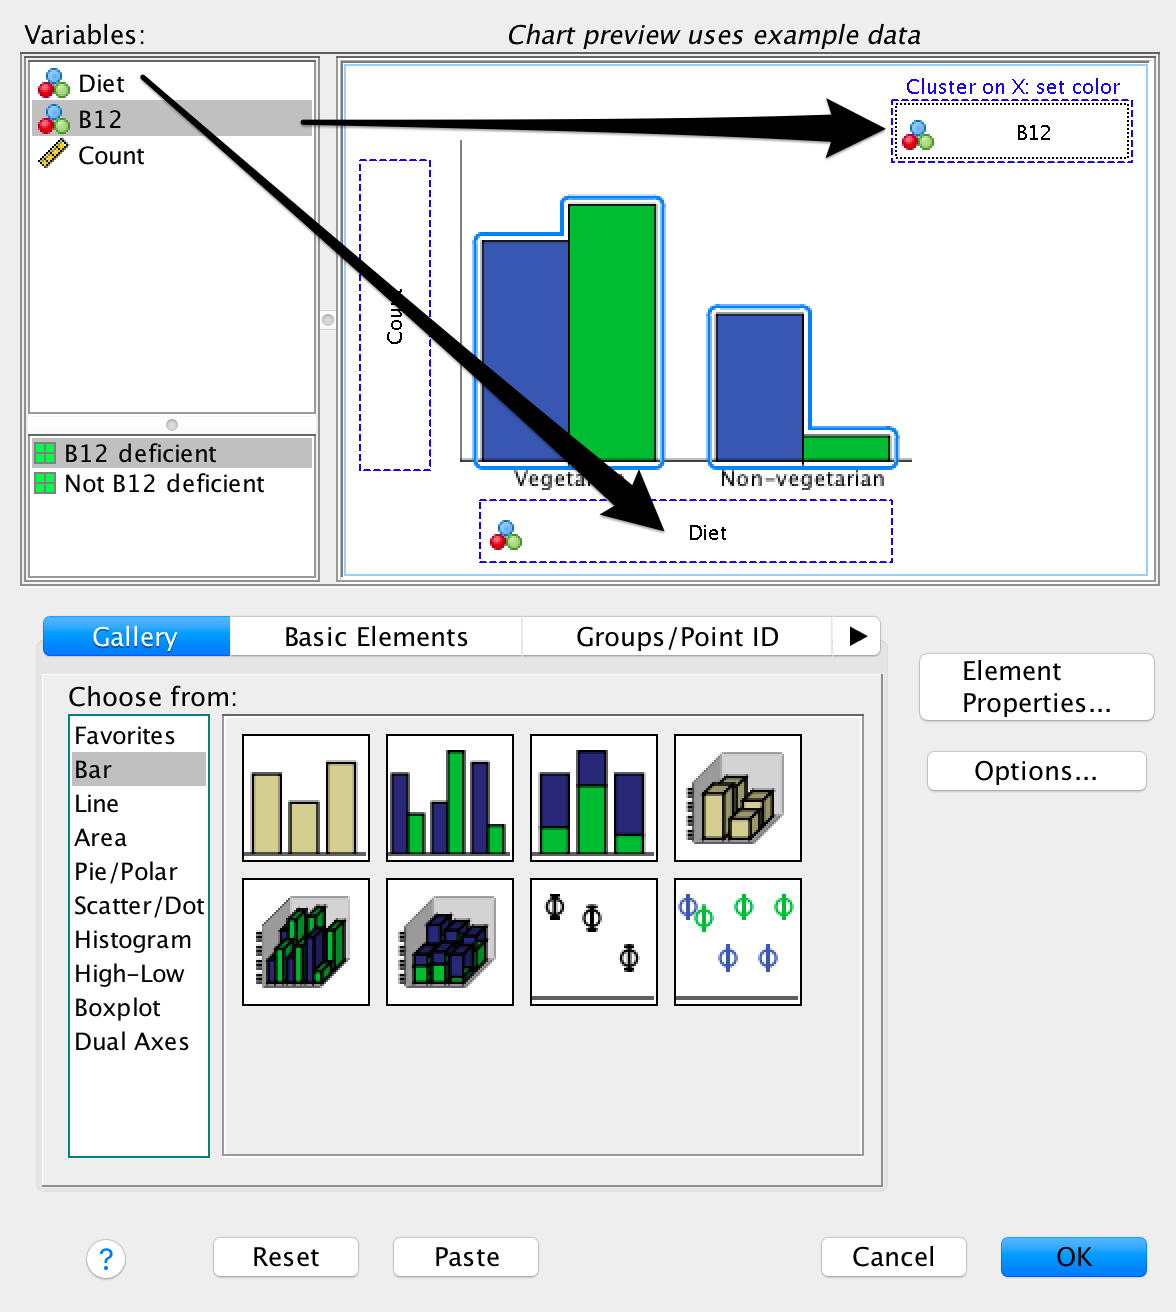
\includegraphics[width=0.85\linewidth]{SPSSImages/Chisq/B12-GraphicsWindows-VarsEntered2} 

}

\caption{Adding the variables to create a side-by-side bar chart}\label{fig:SPSSGraphSbSAddVars}
\end{figure}

\section{Stacked bar charts}\label{SPSSStacked}

For this section, the data introduced in Sect. \ref{SPSSB12Data} are used.

\begin{enumerate}
\def\labelenumi{\arabic{enumi}.}
\tightlist
\item
  \textbf{Use the SPSS menu:} select \textbf{Graphs\textgreater{} Chart Builder\ldots{}}
\item
  \textbf{Select the type of plot}.
  Select \textbf{Bar}, then select the \textbf{third} template from the top row, and drag it to the canvas (Fig.~\ref{fig:SPSSGraphSB}).
\end{enumerate}

\begin{figure}[hbtp]

{\centering 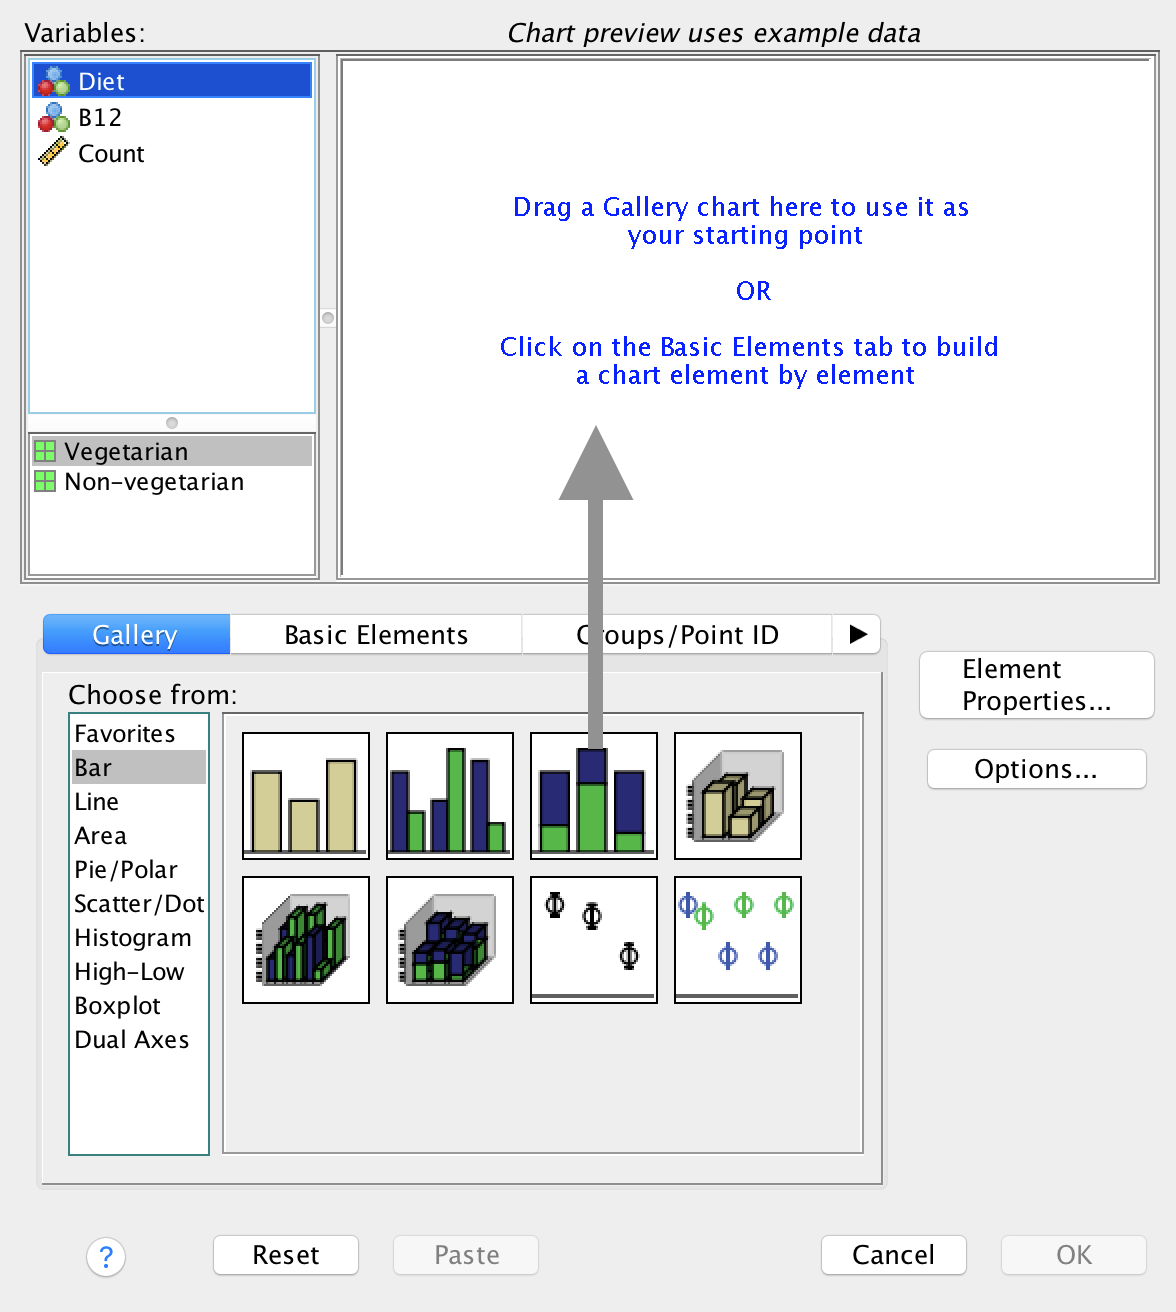
\includegraphics[width=0.85\linewidth]{SPSSImages/Chisq/B12-GraphicsWindow-Stacked} 

}

\caption{Selecting a stacked bar chart}\label{fig:SPSSGraphSB}
\end{figure}

\begin{enumerate}
\def\labelenumi{\arabic{enumi}.}
\setcounter{enumi}{2}
\tightlist
\item
  \textbf{Add the variables}.
  Drag one qualitative variable to the bottom (left-to-right) axis; this can often be seen as the explanatory variable.
  Drag the other to the top right (where it says, cryptically, \textbf{Stack: set color}); Fig.~\ref{fig:SPSSGraphSBAddVars}.
\item
  Press \textbf{OK}.
  You will have your graph in the SPSS Output window.
\end{enumerate}

\begin{figure}[hbtp]

{\centering 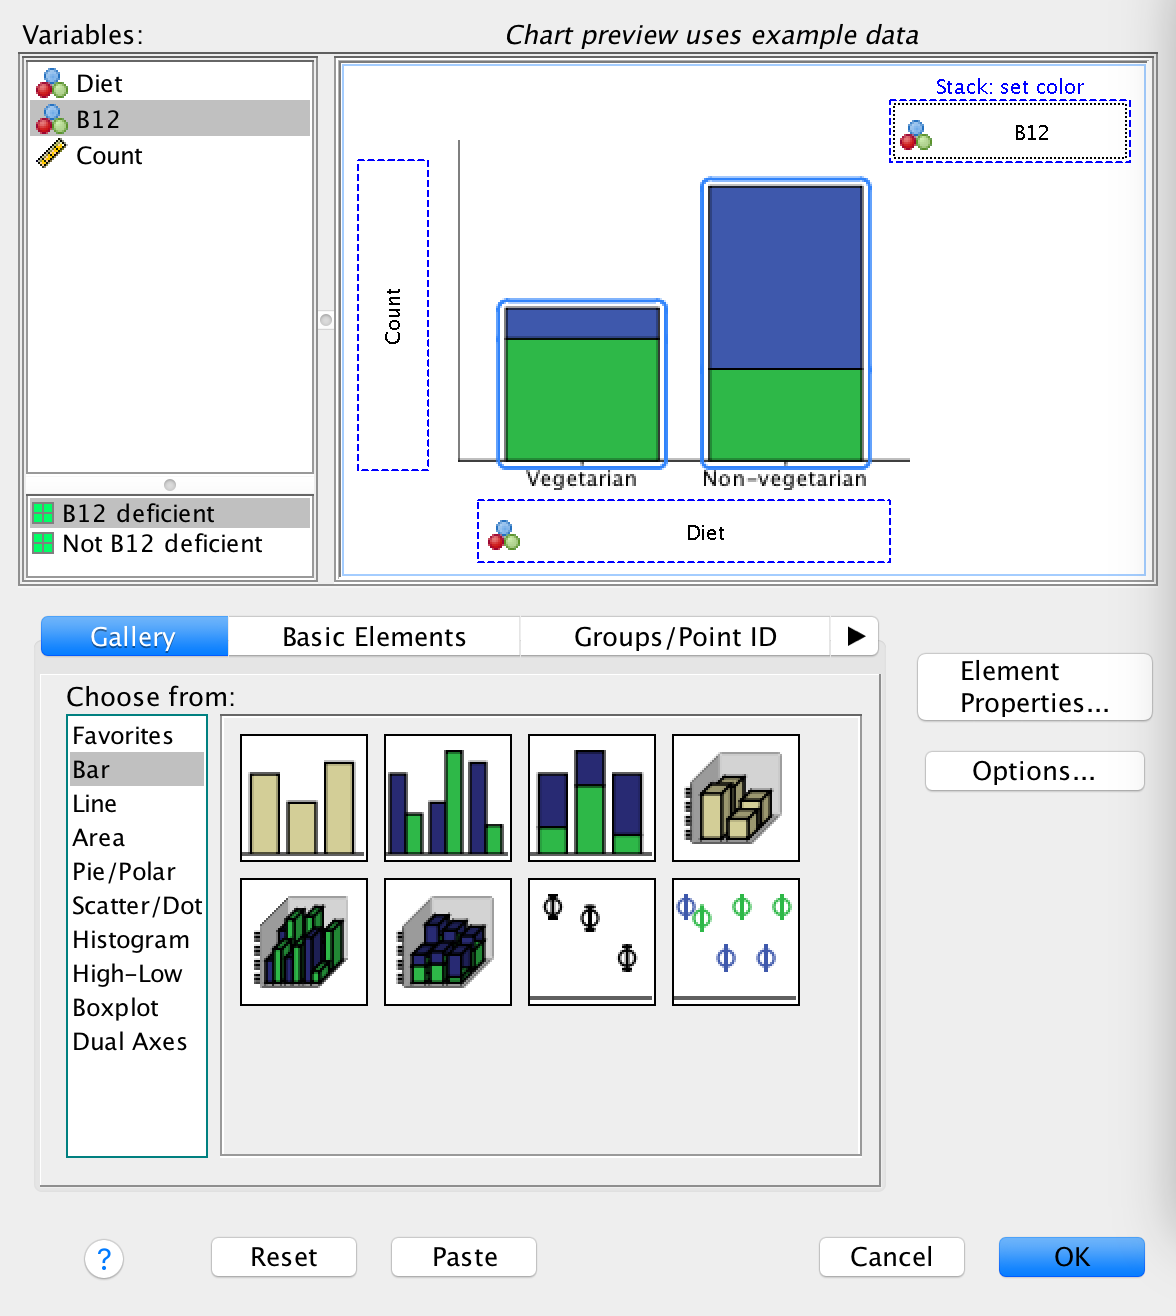
\includegraphics[width=0.85\linewidth]{SPSSImages/Chisq/B12-Stacked-VarsEntered} 

}

\caption{Adding the variables to create a stacked bar chart}\label{fig:SPSSGraphSBAddVars}
\end{figure}

\section{Boxplots}\label{SPSSBoxplot}

For this section, the data introduced in Sect. \ref{SPSSLeanAngle} are used.

\begin{enumerate}
\def\labelenumi{\arabic{enumi}.}
\tightlist
\item
  \textbf{Use the SPSS menu:} select \textbf{Graphs\textgreater{} Chart Builder\ldots{}}
\item
  \textbf{Select the type of plot}.
  Select \textbf{Boxplot}, then select the \textbf{first} template from the top row, and drag it to the canvas (Fig.~\ref{fig:SPSSGraphBoxplotSelect}).
\end{enumerate}

\begin{figure}[hbtp]

{\centering 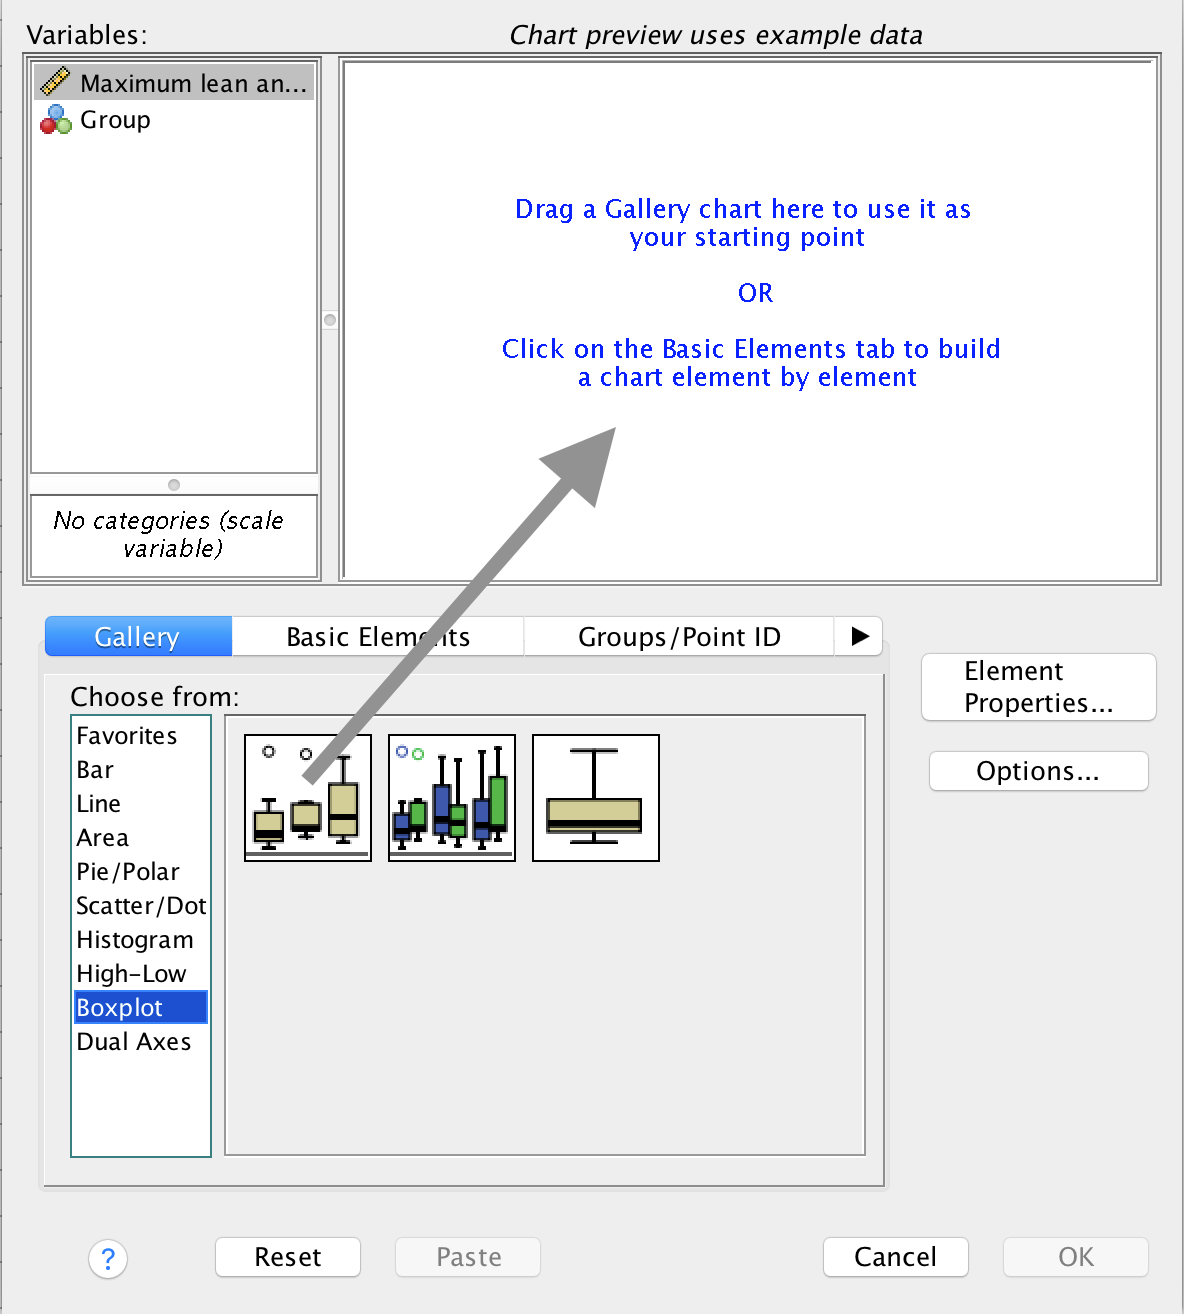
\includegraphics[width=0.85\linewidth]{SPSSImages/Graphics-Boxplot-Drag} 

}

\caption{Selecting a boxplot}\label{fig:SPSSGraphBoxplotSelect}
\end{figure}

\begin{enumerate}
\def\labelenumi{\arabic{enumi}.}
\setcounter{enumi}{2}
\tightlist
\item
  \textbf{Add the variables}.
  Drag the qualitative variable to the bottom (left-to-right) axis; drag the quantitative variable to the vertical (up-and-down) axis (Fig.~\ref{fig:SPSSGraphBoxplotAddVars}).
\item
  Press \textbf{OK}.
  You will have your graph in the SPSS Output window.
\end{enumerate}

\begin{figure}[hbtp]

{\centering 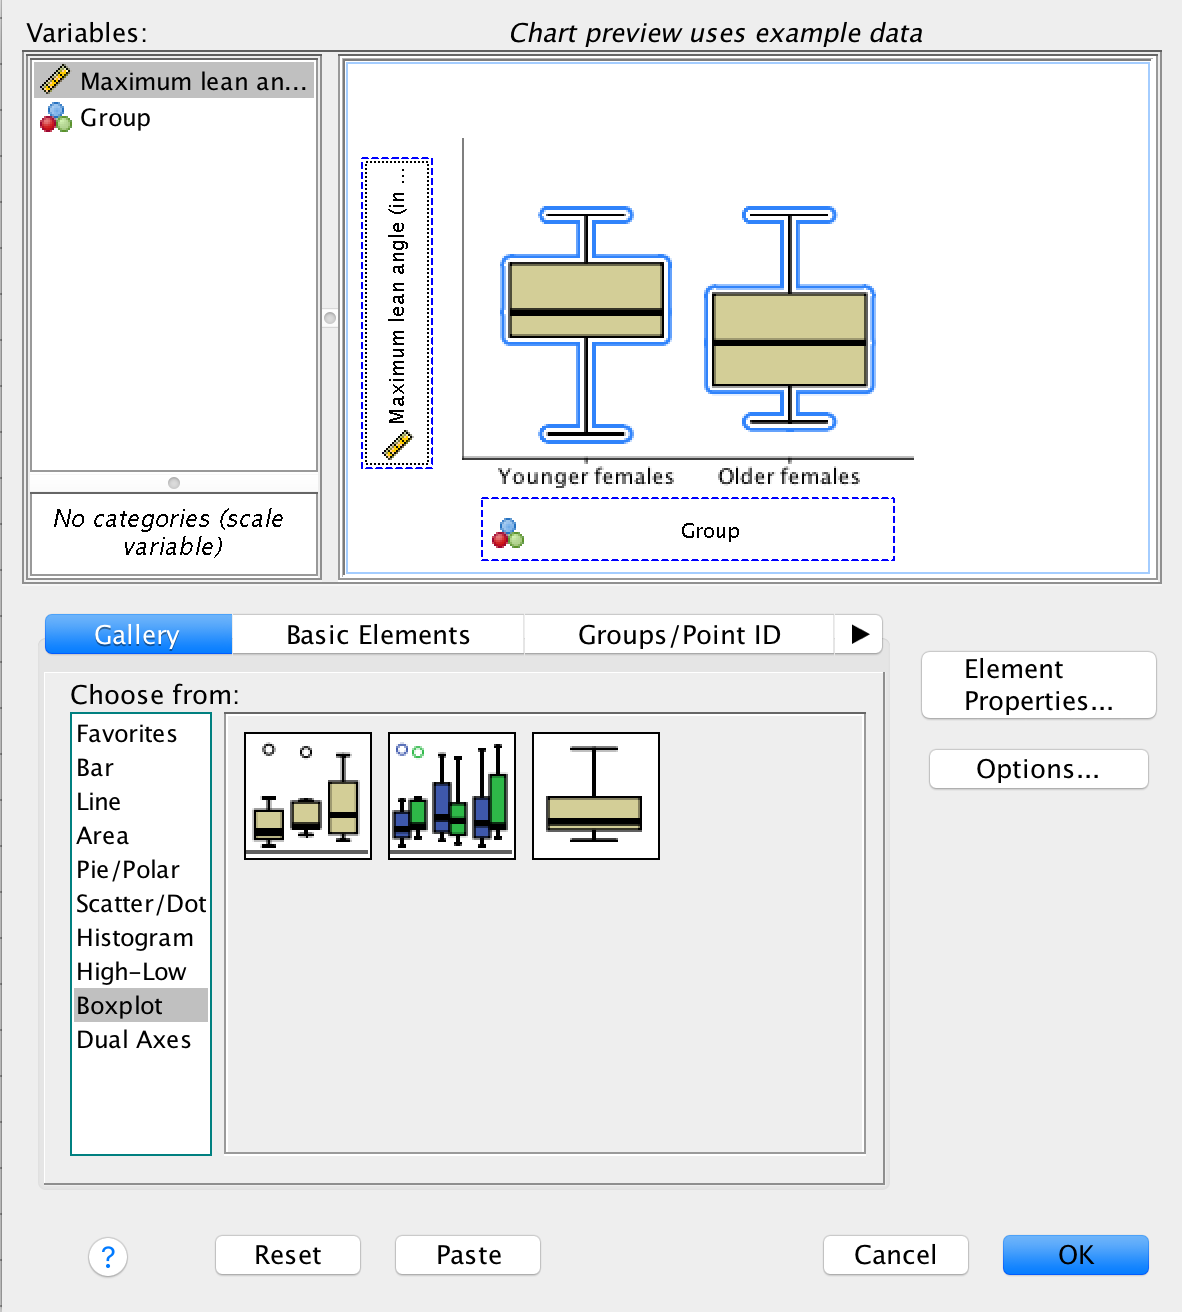
\includegraphics[width=0.85\linewidth]{SPSSImages/Graphics-Boxplot-VarsEntered} 

}

\caption{Adding the variables to create a boxplot}\label{fig:SPSSGraphBoxplotAddVars}
\end{figure}

\section{Error bar charts}\label{SPSSErrorbar}

For this section, the data introduced in Sect. \ref{SPSSLeanAngle} are used.

\begin{enumerate}
\def\labelenumi{\arabic{enumi}.}
\tightlist
\item
  \textbf{Use the SPSS menu:} select \textbf{Graphs\textgreater{} Chart Builder\ldots{}}
\item
  \textbf{Select the type of plot}.
  Select \textbf{Bar}, then select the \textbf{third} template from the \textbf{second row}, and drag it to the canvas (Fig.~\ref{fig:SPSSGraphErrorbarSelect}).
\end{enumerate}

\begin{figure}[hbtp]

{\centering 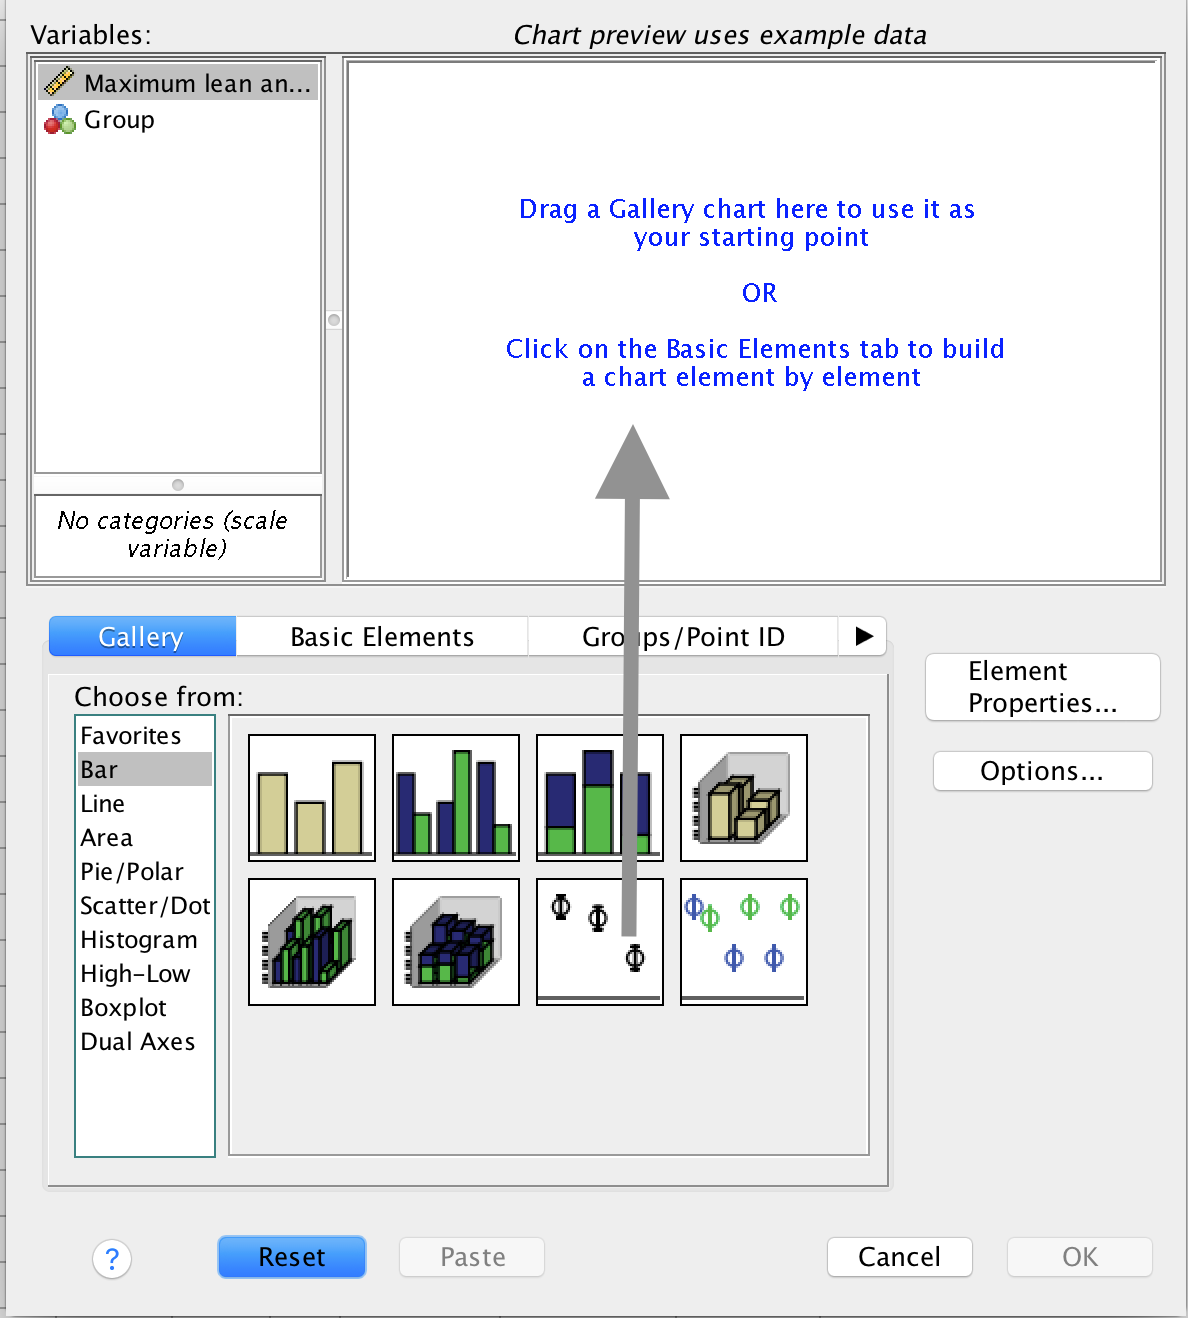
\includegraphics[width=0.85\linewidth]{SPSSImages/Graphics-ErrorBar-Drag} 

}

\caption{Selecting an error bar chart}\label{fig:SPSSGraphErrorbarSelect}
\end{figure}

\begin{enumerate}
\def\labelenumi{\arabic{enumi}.}
\setcounter{enumi}{2}
\tightlist
\item
  \textbf{Add the variables}.
  Drag the qualitative variable to the bottom (left-to-right) axis; drag the quantitative variable to the vertical (up-and-down) axis (Fig.~\ref{fig:SPSSGraphErrorbarAddVars}).
\item
  Press \textbf{OK}.
  You will have your graph in the SPSS Output window.
\end{enumerate}

\begin{figure}[hbtp]

{\centering 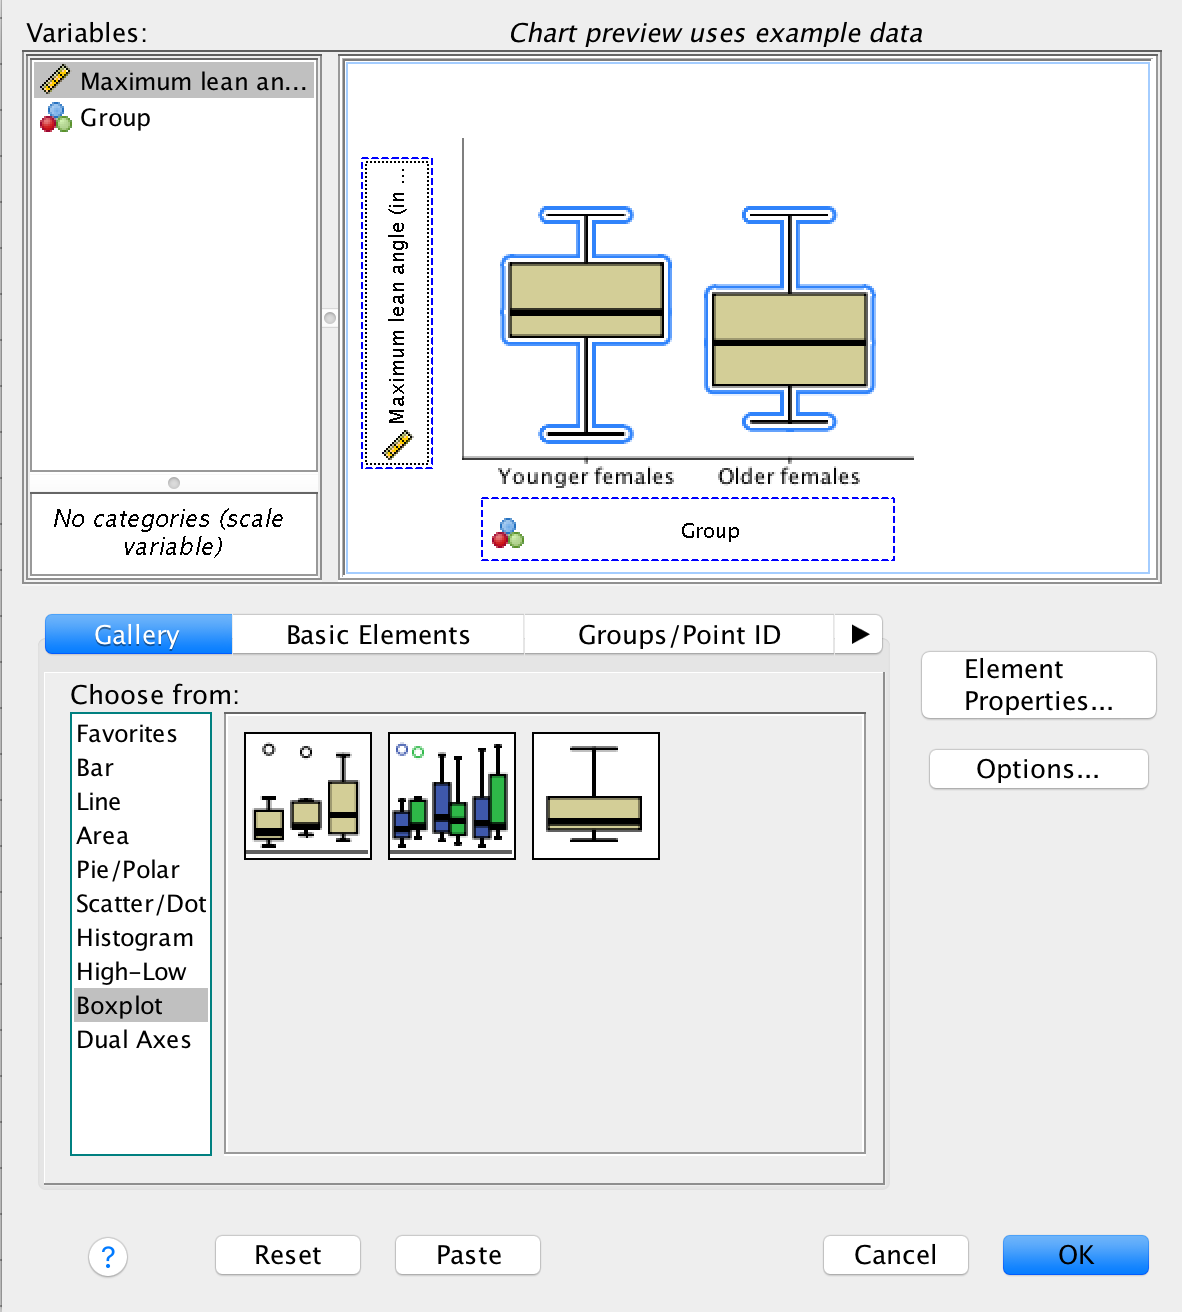
\includegraphics[width=0.85\linewidth]{SPSSImages/Graphics-Boxplot-VarsEntered} 

}

\caption{Adding the variables to create an error bar chart}\label{fig:SPSSGraphErrorbarAddVars}
\end{figure}

\section{Editing graphs}\label{editing-graphs}

Your graph appears in the SPSS Output window.
Double-clicking on the graph opens the \textbf{Chart Editor}.

In the \textbf{Chart Editor}, you can edit almost any part of the graph, by clicking on various elements of the graph (e.g.~the axis labels) or clicking on the icons at the top of the Chart Editor window.

Once you have finished editing your graph in the \textbf{Chart Editor}, close that window, and the graph will be updated in the SPSS Output Window.

\chapter{Data files}\label{DataFiles}

The following data sets are available for download.

\begin{longtable}[]{@{}
  >{\raggedright\arraybackslash}p{(\columnwidth - 6\tabcolsep) * \real{0.1638}}
  >{\centering\arraybackslash}p{(\columnwidth - 6\tabcolsep) * \real{0.1466}}
  >{\centering\arraybackslash}p{(\columnwidth - 6\tabcolsep) * \real{0.2931}}
  >{\centering\arraybackslash}p{(\columnwidth - 6\tabcolsep) * \real{0.3966}}@{}}
\toprule\noalign{}
\begin{minipage}[b]{\linewidth}\raggedright
\textbf{Data}
\end{minipage} & \begin{minipage}[b]{\linewidth}\centering
\textbf{Software}
\end{minipage} & \begin{minipage}[b]{\linewidth}\centering
\textbf{Reference}
\end{minipage} & \begin{minipage}[b]{\linewidth}\centering
\textbf{Download}
\end{minipage} \\
\midrule\noalign{}
\endhead
\bottomrule\noalign{}
\endlastfoot
B12 data & jamovi & Sect. \ref{jamoviChisquare} & \href{./Data/B12-Long.csv}{\texttt{B12-Long.csv}} \\
B12 data & SPSS & Sect. \ref{SPSSOR} & \href{./Data/B12-Long.sav}{\texttt{B12-Long.sav}} \\
Face-plant~data & jamovi & Sect. \ref{jamoviTwoSampleT} & \href{./Data/forwardfall.csv}{\texttt{forwardfall.csv}} \\
Face-plant~data & SPSS & Sect. \ref{SPSSTwoSampleT} & \href{./Data/forwardfall.sav}{\texttt{forwardfall.sav}} \\
\end{longtable}

\chapter*{References}\label{references}


\phantomsection\label{refs}
\begin{CSLReferences}{1}{0}
\bibitem[\citeproctext]{ref-altarawneh2017pilot}
AlTarawneh, Ghada, and Simon Thorne. 2017. {``A Pilot Study Exploring Spreadsheet Risk in Scientific Research.''} \emph{arXiv Preprint arXiv:1703.09785}.

\bibitem[\citeproctext]{ref-berger2007nonstandard}
Berger, Roger L. 2007. {``Nonstandard Operator Precedence in {E}xcel.''} \emph{Computational Statistics \& Data Analysis} 51 (6): 2788--91.

\bibitem[\citeproctext]{ref-mypapers:ScientificResearch}
Dunn, Peter K. 2025. \emph{Scientific Research Methods: An Introduction to Quantitative Research and Statistics}. https://bookdown.org/pkaldunn/SRM-Textbook/.

\bibitem[\citeproctext]{ref-galletta1996spreadsheet}
Galletta, Dennis F., Kathleen S. Hartzel, Susan E. Johnson, Jimmie L. Joseph, and Sandeep Rustagi. 1996. {``Spreadsheet Presentation and Error Detection: An Experimental Study.''} \emph{Journal of Management Information Systems} 13 (3): 45--63.

\bibitem[\citeproctext]{ref-data:Gammon2012:B12}
Gammon, Cheryl S., Pamela R. von Hurst, Joan Coad, Rozanne Kruger, and Welma Stonehouse. 2012. {``Vegetarianism, Vitamin {B12}, and Insulin Resistance in a Group of Predominately Overweight/Obese {S}outh {A}frician Women.''} \emph{Nutrition} 28: 20--24.

\bibitem[\citeproctext]{ref-hargreaves2010polynomial}
Hargreaves, Bruce R., and Thomas P. McWilliams. 2010. {``Polynomial Trendline Function Flaws in {M}icrosoft {E}xcel.''} \emph{Computational Statistics \& Data Analysis} 54 (4): 1190--96.

\bibitem[\citeproctext]{ref-Software:SPSS}
IBM Corp. 2016. \emph{{IBM} {SPSS} Statistics for {W}indows, Version 24.0}. Armonk, NY: {IBM} Corp.

\bibitem[\citeproctext]{ref-keeling2004numerical}
Keeling, Kellie B., and Robert J. Pavur. 2004. {``Numerical Accuracy Issues in Using {E}xcel for Simulation Studies.''} In \emph{Proceedings of the 2004 Winter Simulation Conference, 2004}, 2:1513--18. IEEE.

\bibitem[\citeproctext]{ref-mccullough2002accuracy}
McCullough, B. D., and Berry Wilson. 2002. {``On the Accuracy of Statistical Procedures in {M}icrosoft {E}xcel 2000 and {E}xcel {XP}.''} \emph{Computational Statistics \& Data Analysis} 40 (4): 713--21.

\bibitem[\citeproctext]{ref-melard2014accuracy}
Mélard, Guy. 2014. {``On the Accuracy of Statistical Procedures in {M}icrosoft {E}xcel 2010.''} \emph{Computational Statistics} 29 (5): 1095--1128.

\bibitem[\citeproctext]{ref-panko2016we}
Panko, Ray. 2016. {``What We Don't Know about Spreadsheet Errors Today: The Facts, Why We Don't Believe Them, and What We Need to Do.''} \emph{arXiv Preprint arXiv:1602.02601}.

\bibitem[\citeproctext]{ref-panko1998hitting}
Panko, Raymond R., and Ralph H. Sprague Jr. 1998. {``Hitting the Wall: Errors in Developing and Code Inspecting a {`Simple'} Spreadsheet Model.''} \emph{Decision Support Systems} 22 (4): 337--53.

\bibitem[\citeproctext]{ref-Software:Rsoftware}
R Core Team. 2025. \emph{R: A Language and Environment for Statistical Computing}. Vienna, Austria: R Foundation for Statistical Computing. \url{https://www.R-project.org/}.

\bibitem[\citeproctext]{ref-Software:jamovi}
The jamovi Project. n.d. \emph{{jamovi} (Version 2.5) {[}Computer Software{]}}. \url{https://www.jamovi.org}.

\bibitem[\citeproctext]{ref-data:Wojcik:ForwardFall}
Wojcik, Laura A., Darryl G. Thelen, Albert B. Schultz, James A. Ashton-Miller, and Neil B. Alexander. 1999. {``Age and Gender Differences in Single-Step Recovery from a Forward Fall.''} \emph{Journal of Gerentology} 54A (1): M44--50.

\bibitem[\citeproctext]{ref-ziemann2016gene}
Ziemann, Mark, Yotam Eren, and Assam El-Osta. 2016. {``Gene Name Errors Are Widespread in the Scientific Literature.''} \emph{Genome Biology} 17 (1): 1--3.

\end{CSLReferences}

\backmatter
{\small\printindex}

\end{document}
